\documentclass[preprint, 3p, authoryear]{elsarticle} %review=doublespace preprint=single 5p=2 column
%%% Begin My package additions %%%%%%%%%%%%%%%%%%%

\usepackage[hyphens]{url}

  \journal{An awesome journal} % Sets Journal name

\usepackage{graphicx}
%%%%%%%%%%%%%%%% end my additions to header

\usepackage[T1]{fontenc}
\usepackage{lmodern}
\usepackage{amssymb,amsmath}
% TODO: Currently lineno needs to be loaded after amsmath because of conflict
% https://github.com/latex-lineno/lineno/issues/5
\usepackage{lineno} % add
\usepackage{ifxetex,ifluatex}
\usepackage{fixltx2e} % provides \textsubscript
% use upquote if available, for straight quotes in verbatim environments
\IfFileExists{upquote.sty}{\usepackage{upquote}}{}
\ifnum 0\ifxetex 1\fi\ifluatex 1\fi=0 % if pdftex
  \usepackage[utf8]{inputenc}
\else % if luatex or xelatex
  \usepackage{fontspec}
  \ifxetex
    \usepackage{xltxtra,xunicode}
  \fi
  \defaultfontfeatures{Mapping=tex-text,Scale=MatchLowercase}
  \newcommand{\euro}{€}
\fi
% use microtype if available
\IfFileExists{microtype.sty}{\usepackage{microtype}}{}
\usepackage[]{natbib}
\bibliographystyle{plainnat}

\ifxetex
  \usepackage[setpagesize=false, % page size defined by xetex
              unicode=false, % unicode breaks when used with xetex
              xetex]{hyperref}
\else
  \usepackage[unicode=true]{hyperref}
\fi
\hypersetup{breaklinks=true,
            bookmarks=true,
            pdfauthor={},
            pdftitle={Advancements in Automated Disease Outbreak Detection: A Comparative Simulation Study of a Novel Method against State-of-the-Art Approaches},
            colorlinks=false,
            urlcolor=blue,
            linkcolor=magenta,
            pdfborder={0 0 0}}

\setcounter{secnumdepth}{5}
% Pandoc toggle for numbering sections (defaults to be off)

% Pandoc syntax highlighting
\usepackage{color}
\usepackage{fancyvrb}
\newcommand{\VerbBar}{|}
\newcommand{\VERB}{\Verb[commandchars=\\\{\}]}
\DefineVerbatimEnvironment{Highlighting}{Verbatim}{commandchars=\\\{\}}
% Add ',fontsize=\small' for more characters per line
\usepackage{framed}
\definecolor{shadecolor}{RGB}{248,248,248}
\newenvironment{Shaded}{\begin{snugshade}}{\end{snugshade}}
\newcommand{\AlertTok}[1]{\textcolor[rgb]{0.94,0.16,0.16}{#1}}
\newcommand{\AnnotationTok}[1]{\textcolor[rgb]{0.56,0.35,0.01}{\textbf{\textit{#1}}}}
\newcommand{\AttributeTok}[1]{\textcolor[rgb]{0.13,0.29,0.53}{#1}}
\newcommand{\BaseNTok}[1]{\textcolor[rgb]{0.00,0.00,0.81}{#1}}
\newcommand{\BuiltInTok}[1]{#1}
\newcommand{\CharTok}[1]{\textcolor[rgb]{0.31,0.60,0.02}{#1}}
\newcommand{\CommentTok}[1]{\textcolor[rgb]{0.56,0.35,0.01}{\textit{#1}}}
\newcommand{\CommentVarTok}[1]{\textcolor[rgb]{0.56,0.35,0.01}{\textbf{\textit{#1}}}}
\newcommand{\ConstantTok}[1]{\textcolor[rgb]{0.56,0.35,0.01}{#1}}
\newcommand{\ControlFlowTok}[1]{\textcolor[rgb]{0.13,0.29,0.53}{\textbf{#1}}}
\newcommand{\DataTypeTok}[1]{\textcolor[rgb]{0.13,0.29,0.53}{#1}}
\newcommand{\DecValTok}[1]{\textcolor[rgb]{0.00,0.00,0.81}{#1}}
\newcommand{\DocumentationTok}[1]{\textcolor[rgb]{0.56,0.35,0.01}{\textbf{\textit{#1}}}}
\newcommand{\ErrorTok}[1]{\textcolor[rgb]{0.64,0.00,0.00}{\textbf{#1}}}
\newcommand{\ExtensionTok}[1]{#1}
\newcommand{\FloatTok}[1]{\textcolor[rgb]{0.00,0.00,0.81}{#1}}
\newcommand{\FunctionTok}[1]{\textcolor[rgb]{0.13,0.29,0.53}{\textbf{#1}}}
\newcommand{\ImportTok}[1]{#1}
\newcommand{\InformationTok}[1]{\textcolor[rgb]{0.56,0.35,0.01}{\textbf{\textit{#1}}}}
\newcommand{\KeywordTok}[1]{\textcolor[rgb]{0.13,0.29,0.53}{\textbf{#1}}}
\newcommand{\NormalTok}[1]{#1}
\newcommand{\OperatorTok}[1]{\textcolor[rgb]{0.81,0.36,0.00}{\textbf{#1}}}
\newcommand{\OtherTok}[1]{\textcolor[rgb]{0.56,0.35,0.01}{#1}}
\newcommand{\PreprocessorTok}[1]{\textcolor[rgb]{0.56,0.35,0.01}{\textit{#1}}}
\newcommand{\RegionMarkerTok}[1]{#1}
\newcommand{\SpecialCharTok}[1]{\textcolor[rgb]{0.81,0.36,0.00}{\textbf{#1}}}
\newcommand{\SpecialStringTok}[1]{\textcolor[rgb]{0.31,0.60,0.02}{#1}}
\newcommand{\StringTok}[1]{\textcolor[rgb]{0.31,0.60,0.02}{#1}}
\newcommand{\VariableTok}[1]{\textcolor[rgb]{0.00,0.00,0.00}{#1}}
\newcommand{\VerbatimStringTok}[1]{\textcolor[rgb]{0.31,0.60,0.02}{#1}}
\newcommand{\WarningTok}[1]{\textcolor[rgb]{0.56,0.35,0.01}{\textbf{\textit{#1}}}}

% tightlist command for lists without linebreak
\providecommand{\tightlist}{%
  \setlength{\itemsep}{0pt}\setlength{\parskip}{0pt}}

% From pandoc table feature
\usepackage{longtable,booktabs,array}
\usepackage{calc} % for calculating minipage widths
% Correct order of tables after \paragraph or \subparagraph
\usepackage{etoolbox}
\makeatletter
\patchcmd\longtable{\par}{\if@noskipsec\mbox{}\fi\par}{}{}
\makeatother
% Allow footnotes in longtable head/foot
\IfFileExists{footnotehyper.sty}{\usepackage{footnotehyper}}{\usepackage{footnote}}
\makesavenoteenv{longtable}



\usepackage{booktabs}
\usepackage{longtable}
\usepackage{array}
\usepackage{multirow}
\usepackage{wrapfig}
\usepackage{float}
\usepackage{colortbl}
\usepackage{pdflscape}
\usepackage{tabu}
\usepackage{threeparttable}
\usepackage{threeparttablex}
\usepackage[normalem]{ulem}
\usepackage{makecell}
\usepackage{xcolor}



\begin{document}


\begin{frontmatter}

  \title{Advancements in Automated Disease Outbreak Detection: A Comparative Simulation Study of a Novel Method against State-of-the-Art Approaches}
    \author[Epidemiology Research]{Kasper Schou Telkamp%
  \corref{cor1}%
  \fnref{1}}
   \ead{ksst@ssi.dk} 
    \author[Epidemiology Research]{Lasse Engbo Christiansen%
  %
  \fnref{1}}
   \ead{lsec@ssi.dk} 
    \author[Department of Applied Mathematics and Computer Science]{Jan Kloppenborg Møller%
  %
  \fnref{2}}
   \ead{jkmo@dtu.dk} 
      \affiliation[Epidemiology Research]{
    organization={Epidemiology Research, Statens Serum Institut},addressline={Artillerivej 5},city={Copenhagen S},postcode={2300},country={Denmark},}
    \affiliation[Department of Applied Mathematics and Computer Science]{
    organization={Department of Applied Mathematics and Computer Science, Technical University of Denmark},addressline={Asmussens Allé, Building 303B},city={Lyngby},postcode={2800},country={Denmark},}
    \cortext[cor1]{Corresponding author}
    \fntext[1]{This is the first author footnote.}
    \fntext[2]{Another author footnote.}
  
  \begin{abstract}
  \emph{Background}: Here is a long text that tells me about the background of this
  article. I want to make this text long, so I can illustrate how the abstract
  is formatted.
  \emph{Methods}: These methods have been crucial in the development of this outbreak
  detection algorithm.
  \emph{Results}: These results are outstanding and will forever change the way we
  employ statistical outbreak detection.
  \emph{Conclusion}: Please use my method, as it will result in significant
  advancements within disease outbreak detection.
  \end{abstract}
    \begin{keyword}
    generalized mixed effects models \sep hiearchical generalized lionear models \sep outlier \sep outbreak \sep 
    statistical surveillance
  \end{keyword}
  
 \end{frontmatter}

\hypertarget{introduction}{%
\section{Introduction}\label{introduction}}

The fight against infectious disease not only requires proper treatment of patients and implementation of preventive measures but also demands early detection of emerging disease outbreaks. Today epidemiologists and public health professionals utilize a range of tools and methodologies to effectively tackle disease outbreaks. Here, laboratory-based approaches play a crucial role in outbreak investigations and may involve techniques such as molecular epidemiology \citep[\citet{Struelens_2013}]{Honardoost_2018} and, more recently, Whole Genome Sequencing (WGS) \citep[\citet{Baldry_2010}]{Koeser_2012}.

However, in recent years, there has been a growing interest in statistical methods for automated and early detection of disease outbreak. Statistical outbreak detection begins with the identification of an aberrant number of cases of a particular disease within a specific time and space. When an increase in the number of cases is detected, a signal or alarm is raised by the detection method. Subsequently, an epidemiologist assesses the public health relevance of the aberration to determine if further investigation is warranted. These methodologies encompass various statistical techniques, including regression analysis, time series methodology, methods inspired by statistical process control, approaches incorporating spatial information, and multivariate outbreak detection. A comprehensive review of these methods can be found in studies by \citet{Buckeridge_2007} and \citet{Unkel_2012}.

To establish a golden standard, this article will focus on the method initially proposed by \citet{Farrington_1996} and the subsequent improvements proposed by \citet{Noufaily_2013}. These methods offer advanced statistical tools for detecting and monitoring disease outbreaks and are currently \emph{the} methods of choice at European public health institutes \citep{Hulth_2010}. They can be accessed through the R package called \texttt{surveillance} developed by \citet{Salmon_2016}. It is a well known fact, that one limitation of these detection algorithms is an occasional lack of specificity, leading to false alarms that can overwhelm the epidemiologists with verification tasks \citep{Bedubourg_2017}. Therefore, in this article, these established methods will be compared to a novel outbreak detection algorithm based on hierarchical models. This article introduces this new algorithm as an innovative approach to outbreak detection and aims to assess its performance in comparison to already existing methods.

While hierarchical models have earned a reputation within ecology \citep[\citet{Zuur_2009}]{Bolker_2009}, urban energy modeling \citep[\citet{Jaume_2022}]{Real_2021}, and other fields, their application in the automatic detection of disease outbreaks is relatively unproved. However, there is a promising paper by \citet{Heisterkamp_2006} that applied a hierarchical time series model to detect infectious disease outbreaks in empirical data from \emph{Rubella} and \emph{Salmonella}. The authors concluded that the method is a powerful and versatile way of analyzing time series of routinely recorded laboratory data. In the context of this article, the focus will be on the prospective detection of disease outbreaks, considering the potential of hierarchical models to effectively identify and respond to emerging outbreaks in a timely manner.

\hypertarget{novel-outbreak-detection-algorithm}{%
\section{Novel outbreak detection algorithm}\label{novel-outbreak-detection-algorithm}}

The novel algorithm utilizes a generalized mixed effects model or a hierarchical generalized linear model as a modeling framework to model the count observations \(y\) and assess the unobserved random effects \(u\). These random effects are used directly in the detection algorithm to characterize an outbreak. The theoretical foundations of these models will be further discussed in Sections \ref{glmm} and \ref{hglm}.

The first step involves fitting either a hierarchical Poisson Normal or Poisson Gamma model with a log link to the reference data. Here, it is possible to include an arbitrary number of covariates by supplying a model formula. In order to account for structural changes in the time series, e.g.~an improved and more sensitive diagnostic method or a new screening strategy at hospitals, a rolling window with width \(k\) is used to estimate the time-varying model parameters. Also, it is assumed that the count is proportional to the population size \(n\). Hence in terms of the canonical link the model for the fixed effects is

\begin{equation}
  \log(\lambda_{it}) = x_{it}\beta + \log(n_{it}), \quad i=1,\dots,m, \quad t=1,\dots,T
\end{equation}

Here \(x_{it}\) and \(\beta\) are \(p\)-dimensional vectors of covariates and fixed effects parameters respectively, where \(p\) denotes the number of covariates or fixed effects parameters, \(m\) denotes the number of groups, and \(T\) denotes the length of the period.

In the second step of the algorithm, as a new observation becomes available, the algorithm infers the one-step ahead random effect \(u_{it_1}\) for each group using the obtained model estimates \(\theta_{t_0}\). Here, \(t_0\) represents the current time point, and \(t_1\) represent the one-step ahead time points. The threshold \(U_{t_0}\) for detecting outbreak signals is defined as a quantile of the distribution of random effects in the second stage model. This threshold can be calculated based on either a Gaussian distribution using the plug-in estimate \(\hat{\sigma}_{t_0}\) or a Gamma distribution using the plug-in estimate \(\hat{\phi}_{t_0}\). The choice of distribution depends on the specific modeling framework and assumptions used in the analysis.

In the final step, the inferred random effect \(\hat{u}_{it_1}\) is compared to the upper bound \(U_{t_0}\), and an alarm is raised if \(\hat{u}_{it_1}>U_{t_0}\). If an outbreak is detected, the related observation \(y_{it_1}\) is omitted from the parameter estimation in the future. Thus, resulting in a smaller sample size for the rolling window until that specific observation is discarded.

\hypertarget{generalized-mixed-effects-models}{%
\subsection{\texorpdfstring{Generalized mixed effects models \label{glmm}}{Generalized mixed effects models }}\label{generalized-mixed-effects-models}}

The generalized mixed effects model can be represented by its likelihood function

\begin{equation}\label{eq:glmm}
  L_{M}(\theta; y)=\int_{\mathbb{R}^{q}} L(\theta;u,y) du
\end{equation}

where \(y\) is the observed random variable, \(\theta\) is the model parameters to be estimated and \(U\) is the \(q\) unobserved random variables. The likelihood function \(L\) is the joint likelihood of both the observed and the unobserved random variables. The likelihood function for estimating \(\theta\) is the marginal likelihood \(L_{M}\) obtained by integrating out the unobserved random variables. In general it is difficult to solve the integral in \eqref{eq:glmm} if the number of unobserved random variables is more than a few and hence numerical methods must be used. Thus, an outline of the Laplace approximation is included in this section.

\hypertarget{hiearchical-models}{%
\subsubsection{Hiearchical models}\label{hiearchical-models}}

It is useful to formulate the model as a hierarchical model containing a \emph{first stage model}

\begin{equation}\label{eq:firstStage}
  f_{Y|u}(y;u,\beta)
\end{equation}

which is a model for the observed random variables given the unobserved random variables, and a \emph{second stage model}

\begin{equation}\label{eq:secondStage}
  f_{U}(u; \Psi)
\end{equation}

which is a model for the unobserved random variables. Here \(\beta\) represent the fixed effects parameters and \(\Psi\) is a model parameter. The total set of parameters is \(\theta=(\beta, \Psi)\). Hence the joint likelihood is given as

\begin{equation}\label{eq:jl}
  L(\beta, \Psi; u, y)=f_{Y|u}(y;u,\beta) f_{U}(u; \Psi)
\end{equation}

To obtain the likelihood for the model parameters \((\beta, \Psi)\) the unobserved random variables are integrated out. The likelihood function for estimating \((\beta, \Psi)\) is as in \eqref{eq:glmm} the marginal likelihood

\begin{equation}\label{eq:glmm2}
  L_{M}(\beta, \Psi; y)=\int_{\mathbb{R}^{q}} L(\beta, \Psi;u,y) du
\end{equation}

where \(q\) is the number of unobserved random variables, and \(\beta\) and \(\Psi\) are the parameters to be estimated.

\hypertarget{laplace-approximation}{%
\subsubsection{Laplace approximation}\label{laplace-approximation}}

The Laplace approximation will be outlined in the following. A thorough description of the Laplace approximation in nonlinear mixed effects models is found in \citet{Wolfinger_1997}.

For a given set of model parameters \(\theta\) the joint log-likelihood \(\ell(\theta, u, y)=\log\big(L(\theta, u, y)\big)\) is approximated using a second order Taylor approximation around the optimum \(\tilde{u}=\hat{u}_\theta\) of the log-likelihood function w.r.t. the unobserved random variables \(u\), i.e.,

\begin{equation}\label{eq:laplaceApprox}
  \ell(\theta, u, y)\approx\ell(\theta, \tilde{u}, y) - \frac{1}{2}(u-\tilde{u})^T H(\tilde{u})(u-\tilde{u})
\end{equation}

where the first-order term of the Taylor expansion disappears since the expansion is done around the optimum \(\tilde {u}\) and \(H(\tilde{u})=-\ell_{uu}''(\theta, u, y)|_{u=\tilde{u}}\) is the negative Hessian of the joint log-likelihood evaluated at \(\tilde{u}\).

It is readily seen that the joint log-likelihood for the hierarchical model specified in \ref{eq:firstStage} and \ref{eq:secondStage} is

\begin{equation}
  \ell(\theta, u, y) = \ell(\beta, \Psi, u, y) = \log f_{Y|u}(y;u,\beta)+\log f_U(u;\Psi)
\end{equation}

which implies that the Laplace approximation becomes

\begin{equation}
  \ell_{M,LA}(\theta, y)=\log f_{Y|u}(y; \tilde{u},\beta)+\log f_U(\tilde{u}, \Psi)-\frac{1}{2}\log\Bigg|\frac{H(\tilde{u})}{2\pi}\Bigg|
\end{equation}

\hypertarget{formulation-of-the-generalized-mixed-effects-model}{%
\subsubsection{Formulation of the generalized mixed effects model}\label{formulation-of-the-generalized-mixed-effects-model}}

The generalized mixed effects model utilized in the novel outbreak detection algorithm is formulated as a hierarchical Poisson Normal model. This section presents the joint likelihood function for the first and second stage models.

In order to simplify the notation, the probability density functions are presented for a specific observation. Hence, the subscripts indicating the group and time are omitted. The conditional distribution of the count observations is assumed to be a Poisson distribution with intensities \(\lambda\)

\begin{equation}
  f_{Y|u}(y; u, \beta)=\frac{\lambda\exp(u)^{y}}{y!}\exp\big(-\lambda\exp(u)\big)
\end{equation}

Also, it is assumed that the count is proportional to the population size \(n\). Hence, in terms of the canonical link for the Poisson distribution the model for the fixed effects is

\begin{equation}
\log(\lambda_{it})= x_{it} \beta + \log(n_{it}), \quad i=1,\dots,m, \quad t=1,\dots,T
\end{equation}

The probability density function for the distribution of the random effects is assumed to follow a zero mean Gaussian distribution, \(u\sim\mathrm{N}(0,I\sigma^2)\), i.e.

\begin{equation}
  f_U(u;\sigma)=\frac{1}{\sigma\sqrt{2\pi}}\exp\Bigg(-\frac{u^2}{2\sigma^2}\Bigg)
\end{equation}

where \(\sigma\) is a model parameter.

Henceforth, the total set of parameters are \(\theta=(\beta,\sigma)\) and the model can be formulated as a two-level hierarchical model

\begin{subequations} \label{eq:PoisN}
  \begin{alignat}{2}
    {Y|u} &\sim \mathrm{Pois} \big( \lambda \exp(u) \big) \label{eq:pois_n0} \\ 
    {u} &\sim \mathrm{N}({0},I\sigma^2) \label{eq:pois_n1}
  \end{alignat}
\end{subequations}

The joint likelihood for the count observations \(y\) and the random effects \(u\) becomes

\begin{equation}\label{eq:jnllPoisN}
  L(\beta, \sigma;u_{it},y_{it})=\prod_{t=1}^{T}\prod_{i=1}^{m} \frac{\big(\lambda_{it}\exp(u_{it})\big)^{y_{it}}}{y_{it}!}\exp\big(-\lambda_{it}\exp(u_{it})\big) \prod_{t=1}^{T}\prod_{i=1}^{m} \frac{1}{\sigma\sqrt{2\pi}}\exp\Bigg(-\frac{u_{it}^2}{2\sigma^2}\Bigg)
\end{equation}

\hypertarget{hiearchical-generalized-linear-models}{%
\subsection{\texorpdfstring{Hiearchical generalized linear models \label{hglm}}{Hiearchical generalized linear models }}\label{hiearchical-generalized-linear-models}}

In this section selected theory related to hierarchical generalized linear models is presented. The model class was initially formulated by \citet{Lee_1996} as a natural generalization of the generalized linear model to also incorporate random effects. A starting point in hierarchical modelling is an assumption that the distribution of random effects may be modeled by an exponential dispersion family. This family of models were first introduced by \citet{Fisher_1922}, and has proven to play an important role in mathematical statistics because of their simple inferential properties. The exponential dispersion family considers a family of distributions, which can be written on the form

\begin{equation}\label{eq:expDispFam}
  f_Y(y;\theta)=c(y,\phi)\exp\big(\phi \{\theta y-\kappa(\theta) \}\big)
\end{equation}

Here the parameter \(\phi>0\) is called the \emph{precision parameter}, which in some cases represents a shape parameter as for the Gamma distribution. In other cases the precision parameter represents an over-dispersion that is not related to the mean. These distributions combine with the so-called \emph{standard conjugate distributions} in a simple way, and lead to marginal distributions that may be expressed in a closed form suited for likelihood calculations. For an introduction to the concept of \emph{standard conjugate distributions} and the definition of a hierarchical generalized linear model, refer to Section 6.3 and Section 6.5 of \citet{Madsen_2010}, respectively.

\hypertarget{formulation-of-the-hiearchical-generalzied-linear-model}{%
\subsubsection{Formulation of the hiearchical generalzied linear model}\label{formulation-of-the-hiearchical-generalzied-linear-model}}

The hierarchical generalized linear model used by the novel outbreak detection algorithm is formulated as a hierarchical Poisson Gamma model. This section present the derivation of the marginal distribution of \(Y\) along with the joint likelihood function for the first and second stage models.

In the compound Poisson Gamma model the conditional distribution of the count observations are assumed to be a Poisson distribution with intensities \(\lambda\)

\begin{equation}\label{eq:pdfPois}
  f_{Y|u}(y;u,\beta)=\frac{(\lambda u)^{y}}{y!}\exp(-\lambda u)
\end{equation}

The probability density function for the random effects \(u\) are assumed to follow a reparametrized Gamma distribution with mean \(1\), \(u \sim \mathrm{G}(1/\phi,\phi)\) that is

\begin{equation} \label{eq:pdfGamma}
  f_{u}(u;\phi)=\frac{1}{\phi \Gamma(1/\phi)} \bigg(\frac{u}{\phi}\bigg)^{1/\phi-1} \exp (-u/\phi)
\end{equation}

Subsequently, the model can be formulated as a two-level hierarchical model

\begin{subequations} \label{eq:PoisGam}
  \begin{alignat}{2}
    {Y|u} &\sim \mathrm{Pois} (\lambda u) \label{eq:pois_g0} \\ 
    {u} &\sim \mathrm{G}( 1/\phi,\phi) \label{eq:pois_g1}
  \end{alignat}
\end{subequations}

Given \ref{eq:pdfPois} and \ref{eq:pdfGamma}, the probability function for the marginal distribution of \(Y\) is determined from

\begin{equation} \label{eq:marMix}
  \begin{aligned}
    g_{Y}(y;\beta,\phi)&=\int_{u=0}^\infty f_{Y|u}(y;u,\beta) f_{u}(u;\phi) \,du \\
    &=\int_{u=0}^\infty \frac{(\lambda u)^y}{y!} \exp (-\lambda u) \frac{1}{\phi \Gamma(1/\phi)} \bigg(\frac{u}{\phi}\bigg)^{1/\phi-1} \exp (-u /\phi) \,du\\
    &=\frac{\lambda^{y}}{y!\Gamma(1/\phi)\phi^{1/\phi}} \int_{u=0}^\infty u^{y+1/\phi-1} \exp \big(-u(\lambda \phi+1)/\phi\big) \,du
  \end{aligned}
\end{equation}

In \ref{eq:marMix} it is noted that the integrand is the kernel in the probability density function for a Gamma distribution, \(\mathrm{G}\big(y+1/\phi,\phi/(\lambda \phi+1)\big)\). As the integral of the density shall equal one, it is found by adjusting the norming constant that

\begin{equation}
  \int_{u=0}^\infty  u^{ y+ 1/\phi-1} \exp \Big(- u/\big(\phi/( \lambda \phi+1)\big)\Big) \,du = \frac{\phi^{ y+ 1/\phi}\Gamma( y+ 1/\phi)}{( \lambda \phi + 1)^{y+1/\phi}}
\end{equation}

Therefore, it is shown that the marginal distribution of \(Y\) is a Negative Binomial distribution, \(Y\sim\mathrm{NB}\big(1/\phi,1/(\lambda\phi+1)\big)\). The probability function for \(Y\) is

\begin{equation} \label{eq:pdfMix}
  \begin{aligned}
    P[Y=y]&=g_{Y}(y; \beta, \phi) \\
    &=\frac{\lambda^{y}}{y!\Gamma(1/\phi)\phi^{1/\phi}}\frac{\phi^{y+1/\phi}\Gamma(y+1/\phi)}{(\lambda \phi + 1)^{y+1/\phi}} \\
    &=\frac{\Gamma(y+1/\phi)}{\Gamma(1/\phi)y!}\frac{1}{(\lambda\phi+1)^{1/\phi}}\bigg(\frac{\lambda\phi}{\lambda\phi+1}\bigg)^{y} \\
    &=\begin{pmatrix} y+1/\phi-1 \\ y \end{pmatrix} \frac{1}{(\lambda\phi+1)^{1/\phi}}\bigg(\frac{\lambda\phi}{\lambda\phi+1}\bigg)^{y} \ , \quad \mathrm{for} \ y = 0, 1, 2, \dots
  \end{aligned}
\end{equation}

where the following convention is used

\begin{equation}
  \begin{pmatrix} z\\y \end{pmatrix} = \frac{\Gamma(z+1)}{\Gamma(z+1-y)y!}
\end{equation}

for \(z\) real and \(y\) integer values. Consequently, the mean and variance of \(Y\) are given by

\begin{equation}\label{eq:meanNB}
  \mathrm{E}[Y] = \lambda \qquad \mathrm{V}[Y] = \lambda (\lambda \phi + 1)
\end{equation}

The joint likelihood function for estimating \((\beta,\phi)\) is

\begin{equation}\label{eq:jnllPoisG}
  L( \beta, \phi; y_{it})=\prod_{t=1}^{T}\prod_{i=1}^{m} \begin{pmatrix} y_{it}+1/\phi-1 \\ y_{it} \end{pmatrix} \frac{1}{(\lambda_{it}\phi+1)^{1/\phi}}\bigg(\frac{\lambda_{it}\phi}{\lambda_{it}\phi+1}\bigg)^{y_{it}}
\end{equation}

\hypertarget{inference-on-individual-groups}{%
\subsubsection{Inference on individual groups}\label{inference-on-individual-groups}}

Consider the compound Poisson Gamma model in \ref{eq:PoisGam}, and assume that a value \(Y=y\) has been observed.

The conditional distribution of \(u\) for given \(Y=y\) is found using Bayes Theorem. In order to simplify the notation, the subscript indicating the group and time are omitted.

\begin{equation}
  \begin{aligned}
    g_{u}(u|Y=y)&=\frac{f_{y,u}(y,u)}{g_Y(y;\lambda, \phi)} \\
    &=\frac{f_{y|u}(y;u)g_{u}(u)}{g_{Y}(y;\lambda,\phi)} \\
    &=\frac{1}{g_{Y}(y;\lambda,\phi)}\Bigg(\frac{(\lambda u)^y}{y!} \exp (-\lambda u) \frac{1}{\phi \Gamma(1/\phi)} \bigg(\frac{u}{\phi}\bigg)^{1/\phi-1} \exp (-u/\phi)\Bigg) \\
    &\propto u^{y+1/\phi-1} \exp \big(- u(\lambda\phi+1)/\phi\big)
  \end{aligned}
\end{equation}

Here, the \textit{kernel} of the probability density function is identified

\begin{equation}
  u^{y+1/\phi-1} \exp (- u(\lambda\phi+1)/\phi)
\end{equation}

as the kernel of a Gamma distribution, \(\mathrm{G}(y+1/\phi,\phi/(\lambda\phi+1))\), i.e.~the conditional distribution of \(u\) for given \(Y=y\) can be written as

\begin{equation}
  u| Y=y\sim \mathrm{G}\big(y+1/\phi,\phi/(\lambda \phi+1)\big)
\end{equation}

The mean of the conditional distribution is given by:

\begin{equation}
  \mathrm{E}[u|Y=y]=\frac{y\phi+1}{\lambda \phi+1}
\end{equation}

And the variance of the conditional distribution is:

\begin{equation}
  \mathrm{V}[u|Y=y]=\frac{( \phi^2+\phi)}{(\lambda \phi + 1)^2}
\end{equation}

These formulas provide the mean and variance of the conditional distribution of \(u\) given the observed value \(Y=y\).

\hypertarget{the-rationale-for-employing-the-gamma-distribution-as-a-second-stage-model}{%
\subsubsection{The rationale for employing the Gamma distribution as a second stage model}\label{the-rationale-for-employing-the-gamma-distribution-as-a-second-stage-model}}

The choice of the Gamma distribution for modeling the random effects has been motivated by several reasons. Firstly, the support of the Gamma distribution, which ranges from 0 to infinity, aligns with the mean-value space, denoted as \(\mathcal{M}\), for the Poisson distribution. This ensures that the random effects are constrained within a meaningful range for the underlying Poisson process.

Secondly, the two-parameter family of Gamma distributions offers considerable flexibility, encompassing a wide range of shapes and distributions that can span from exponential-like distributions to fairly symmetrical distributions on the positive real line. This flexibility allows the model to capture various patterns and characteristics observed in the data.

Additionally, the choice of the Gamma distribution has benefits in terms of the derivation of the marginal distribution of the response variable \(Y\). The kernel \(u^{\alpha-1}\exp(-u/\beta)\) of the Gamma distribution used for modeling the random effects exhibits a similar structure to the kernel \(u^y\exp(-u)\) of the likelihood function corresponding to the sampling distribution of \(Y\). This similarity facilitates the analytical computation of the integral involved in deriving the marginal distribution, as it can be expressed in terms of known functions.

Overall, the Gamma distribution is selected due to its alignment with the mean-value space of the Poisson distribution, its flexibility in capturing diverse distributions, and its analytical convenience in computing the marginal distribution of the response variable.

\hypertarget{parameter-estimation}{%
\section{Parameter estimation}\label{parameter-estimation}}

The generalized mixed effect and hierarchical generalized linear models are implemented in R using the open-source R package \texttt{TMB} (Template Model Builder) developed by \citet{Kristensen_2016}. This package facilitates efficient maximum likelihood estimation and uncertainty calculations for the parameter set \(\theta=(\beta, \Psi)\) and random effects \(u\). The presentation of the parameter estimation conducted in \texttt{TMB} is strongly inspired by Chapter 2 in \citet{Kristensen_2016} and Section 5.10 in \citet{Madsen_2010}.

\texttt{TMB} maximizes a user-provided objective function in the form of a C++ template, to estimate the maximum likelihood for the parameter set \(\theta=(\beta, \Psi)\). The following code chunk illustrates the C++ template for the hierarchical Poisson Normal model specified in \ref{eq:PoisN}:

\begin{Shaded}
\begin{Highlighting}[]
\PreprocessorTok{\#include }\ImportTok{\textless{}TMB.hpp\textgreater{}}
\KeywordTok{template}\OperatorTok{\textless{}}\KeywordTok{class}\NormalTok{ Type}\OperatorTok{\textgreater{}}
\NormalTok{Type objective\_function}\OperatorTok{\textless{}}\NormalTok{Type}\OperatorTok{\textgreater{}::}\KeywordTok{operator}\OperatorTok{()} \OperatorTok{()}
\OperatorTok{\{}
  \CommentTok{// R input data}
\NormalTok{  DATA\_VECTOR}\OperatorTok{(}\NormalTok{y}\OperatorTok{);}                               \CommentTok{// Count data}
\NormalTok{  DATA\_VECTOR}\OperatorTok{(}\NormalTok{x}\OperatorTok{);}                               \CommentTok{// Population size}
\NormalTok{  DATA\_MATRIX}\OperatorTok{(}\NormalTok{X}\OperatorTok{);}                               \CommentTok{// Design matrix}
\NormalTok{  PARAMETER\_VECTOR}\OperatorTok{(}\NormalTok{u}\OperatorTok{);}                          \CommentTok{// Random effects}
  \CommentTok{// Parameters}
\NormalTok{  PARAMETER\_VECTOR}\OperatorTok{(}\NormalTok{beta}\OperatorTok{);}                       \CommentTok{// Fixed effects parameters}
\NormalTok{  PARAMETER}\OperatorTok{(}\NormalTok{log\_sigma\_u}\OperatorTok{);}                       \CommentTok{// Model parameter}
\NormalTok{  vector}\OperatorTok{\textless{}}\NormalTok{Type}\OperatorTok{\textgreater{}}\NormalTok{ lambda  }\OperatorTok{=}\NormalTok{ exp}\OperatorTok{(}\NormalTok{X}\OperatorTok{*}\NormalTok{beta}\OperatorTok{{-}}\NormalTok{log}\OperatorTok{(}\NormalTok{x}\OperatorTok{)+}\NormalTok{u}\OperatorTok{);}  \CommentTok{// Construct \textquotesingle{}lambda\textquotesingle{}}
\NormalTok{  Type sigma\_u }\OperatorTok{=}\NormalTok{ exp}\OperatorTok{(}\NormalTok{log\_sigma\_u}\OperatorTok{);}              \CommentTok{// And the model parameters}
\NormalTok{  Type mean\_ran }\OperatorTok{=}\NormalTok{ Type}\OperatorTok{(}\DecValTok{0}\OperatorTok{);}
  \CommentTok{// Objective function}
\NormalTok{  Type f }\OperatorTok{=} \DecValTok{0}\OperatorTok{;}                                   \CommentTok{// Declare the objective}
\NormalTok{  f }\OperatorTok{{-}=}\NormalTok{ sum}\OperatorTok{(}\NormalTok{dnorm}\OperatorTok{(}\NormalTok{u}\OperatorTok{,}\NormalTok{mean\_ran}\OperatorTok{,}\NormalTok{sigma\_u}\OperatorTok{,}\KeywordTok{true}\OperatorTok{));}     \CommentTok{// Calculate the objective}
\NormalTok{  f }\OperatorTok{{-}=}\NormalTok{ sum}\OperatorTok{(}\NormalTok{dpois}\OperatorTok{(}\NormalTok{y}\OperatorTok{,}\NormalTok{lambda}\OperatorTok{,}\KeywordTok{true}\OperatorTok{));}               \CommentTok{// Calculate the objective}
  \ControlFlowTok{return}\NormalTok{ f}\OperatorTok{;}
\OperatorTok{\}}
\end{Highlighting}
\end{Shaded}

The objective function maximizes the marginal log-likelihood function, which integrates out the random effects \(u\)

\begin{equation}
  \ell_{M}(\theta; y)=\int_{\mathbb{R}^{q}} \ell (\theta;u,y) du
\end{equation}

where \(\ell(\theta, u,y)\) is the joint log-likelihood function of the data given the parameters and random effects. The maximizer \(\hat{u}_{\theta}\) of the joint log-likelihood \(\ell(\theta;u,y)\) with respect to the random effects \(u\) is defined as:

\begin{equation}
  \hat{u}_{\theta}=\mathop{\mathrm{arg\,max}}_{u} \ell(\theta;u,y)
\end{equation}

Using \(H(\hat{u}_{\theta})\) to denote the negative Hessian of the joint log-likelihood evaluated at \(\hat{u}_{\theta}\); i.e,

\begin{equation}
  H(\hat{u}_{\theta}) =-\ell_{uu}''(\theta, u, y)|_{u=\hat{u}_{\theta}}
\end{equation}

The Laplace approximation for the marginal log-likelihood \(\ell_M(\theta)\) is

\begin{equation}
  \ell_{M,LA}(\theta, y)=\ell(\theta,u,y)-\frac{1}{2}\log \Big|\frac{H(\hat{u}_{\theta})}{2\pi}\Big|
\end{equation}

Our estimate of \(\theta\) minimizes the negative log of the Laplace approximation, i.e.,

\begin{equation}
  \hat{\theta}=\mathop{\mathrm{arg\,min}}_{\theta} - \ell_{M, LA}(\theta, y)
\end{equation}

The minimization of the Laplace approximation for the marginal likelihood is then performed using conventional R optimization routines (e.g., BFGS) to optimize the objective and obtain our estimate \(\hat{\theta}\). Uncertainty of the estimate \(\hat{\theta}\), or any differentiable function of the estimate \(\phi(\hat{\theta})\), is obtained by the \(\delta\)-method:

\begin{equation}
  \mathrm{V}\big(\phi(\hat{\theta})\big)=-\phi_{\theta}'(\hat{\theta})\Big(\Delta^2 \ell_{M,LA}(\hat{\theta}, y)\Big)^{-1} \phi_{\theta}'(\hat{\theta})^T
\end{equation}

Additionally, \texttt{TMB} utilizes Automatic Differentiation (AD) techniques \citep{Griewank_2008} to evaluate first, second, and potentially third-order derivatives. This approach enhances the computational efficiency and accuracy of the parameter estimation process in the implemented models. Therefore, even though the random effects are analytically integrated out in the hierarchical Poisson Gamma model, and the Laplace approximation is not needed, implementing the joint log-likelihood function in \texttt{TMB} can still result in more efficient computations. For a comprehensive introduction to the concept of AD, it is recommended to read Section 2.1 and Section 2.2 of \citet{Fournier_2012}.

\hypertarget{simulation-study}{%
\section{Simulation study}\label{simulation-study}}

This subsection includes a thorough description of the simulation study conducted to evaluate the performance of the novel outbreak detection algorithm compared to state-of-the-art algorithms. The simulations cover various scenarios, adapted from the study by \citet{Noufaily_2013}, and are investigated using varying significance levels, \(\alpha\), for the threshold calculations. In this article, the following set of significance levels are investigated for each of the methods: \(\alpha=\{0.005, 0.01 0.025, 0.05, 0.1\}\).

The subsection begins by describing the method used to simulate the baseline data. These data are generated using a Negative Binomial model with a time-dependent mean \(\mu(t)\). Next, the assumptions regarding the simulated outbreaks are outlined, including the outbreak size and distribution in time.

The evaluation measures used to assess the performance of the outbreak detection algorithms are then presented. These measures are designed to capture relevant quantities in the context of outbreak detection.

\hypertarget{the-simulated-baseline-data}{%
\subsection{The simulated baseline data}\label{the-simulated-baseline-data}}

The simulated baseline data is generated using a Negative Binomial model with a mean parameter \(\mu\) and a variance parameter \(\phi\mu\). The dispersion parameter \(\phi\) is assumed to be greater than or equal to 1. The mean \(\mu(t)\) is defined by a linear predictor that includes a trend component and a seasonality component represented by Fourier terms.

The equation for \(\mu(t)\) is given as:

\begin{equation}
  \mu(t)=\exp\Biggl(\theta+\beta_t+\sum_{j=1}^m \biggl(\gamma_1 \cos\Bigl(\frac{2\pi jt}{52}\Bigl) + \gamma_2 \sin \Bigl(\frac{2\pi jt}{52} \Bigl)\biggl)\Biggl)
\end{equation}

In this equation, \(m\) represents the number of Fourier terms used to model seasonality. When \(m=0\), it indicates the absence of seasonality, while \(m=1\) corresponds to annual seasonality.

To cover a wide range of data sets encountered in practical applications, 28 different parameter combinations are generated. These combinations vary in terms of trends (represented by different values of \(\beta\)), seasonalities (represented by different values of \(\gamma_1\) and \(\gamma_2\)), baseline frequencies of reports (represented by different values of \(\theta\)), and dispersion (represented by different values of \(\phi\)). The specific parameter values for the 28 scenarios are provided in Table \ref{tab:scenariosTbl}.

\begin{longtable}[t]{llllllll}
\caption{\label{tab:scenariosTbl}Parameters and criteria utilized to generate the 28 scenarios.}\\
\toprule
Scenario & $\theta$ & $\phi$ & $\beta$ & $\gamma_1$ & $\gamma_2$ & $m$ & Trend\\
\midrule
\endfirsthead
\caption[]{\textit{(continued)}}\\
\toprule
Scenario & $\theta$ & $\phi$ & $\beta$ & $\gamma_1$ & $\gamma_2$ & $m$ & Trend\\
\midrule
\endhead

\endfoot
\bottomrule
\endlastfoot
1 & 0.10 & 1.5 & 0.0000 & 0.00 & 0.00 & 0 & 0\\
2 & 0.10 & 1.5 & 0.0000 & 0.60 & 0.60 & 1 & 0\\
3 & 0.10 & 1.5 & 0.0025 & 0.00 & 0.00 & 0 & 1\\
4 & 0.10 & 1.5 & 0.0025 & 0.60 & 0.60 & 1 & 1\\
\addlinespace
5 & -2.00 & 2.0 & 0.0000 & 0.00 & 0.00 & 0 & 0\\
6 & -2.00 & 2.0 & 0.0000 & 0.10 & 0.30 & 1 & 0\\
7 & -2.00 & 2.0 & 0.0050 & 0.00 & 0.00 & 0 & 1\\
8 & -2.00 & 2.0 & 0.0050 & 0.10 & 0.30 & 1 & 1\\
\addlinespace
9 & 1.50 & 1.0 & 0.0000 & 0.00 & 0.00 & 0 & 0\\
10 & 1.50 & 1.0 & 0.0000 & 0.20 & -0.40 & 1 & 0\\
11 & 1.50 & 1.0 & 0.0030 & 0.00 & 0.00 & 0 & 1\\
12 & 1.50 & 1.0 & 0.0030 & 0.20 & -0.40 & 1 & 1\\
\addlinespace
13 & 0.50 & 5.0 & 0.0000 & 0.00 & 0.00 & 0 & 0\\
14 & 0.50 & 5.0 & 0.0000 & 0.50 & 0.50 & 1 & 0\\
15 & 0.50 & 5.0 & 0.0020 & 0.00 & 0.00 & 0 & 1\\
16 & 0.50 & 5.0 & 0.0020 & 0.50 & 0.50 & 1 & 1\\
\addlinespace
17 & 2.50 & 3.0 & 0.0000 & 0.00 & 0.00 & 0 & 0\\
18 & 2.50 & 3.0 & 0.0000 & 1.00 & 0.10 & 1 & 0\\
19 & 2.50 & 3.0 & 0.0010 & 0.00 & 0.00 & 0 & 1\\
20 & 2.50 & 3.0 & 0.0010 & 1.00 & 0.10 & 1 & 1\\
\addlinespace
21 & 3.75 & 1.1 & 0.0000 & 0.00 & 0.00 & 0 & 0\\
22 & 3.75 & 1.1 & 0.0000 & 0.10 & -0.10 & 1 & 0\\
23 & 3.75 & 1.1 & 0.0010 & 0.00 & 0.00 & 0 & 1\\
24 & 3.75 & 1.1 & 0.0010 & 0.10 & -0.10 & 1 & 1\\
\addlinespace
25 & 5.00 & 1.2 & 0.0000 & 0.00 & 0.00 & 0 & 0\\
26 & 5.00 & 1.2 & 0.0000 & 0.05 & 0.01 & 1 & 0\\
27 & 5.00 & 1.2 & 0.0001 & 0.00 & 0.00 & 0 & 1\\
28 & 5.00 & 1.2 & 0.0001 & 0.05 & 0.01 & 1 & 1\\*
\end{longtable}

To simulate the baseline data without outbreaks, 100 replicates are generated for each of the 28 parameter scenarios. Each replicate consist of a time series of size \(T=624\) weeks.

The 624 weeks are divided into three periods: weeks 1-313 are used for training, weeks 313-575 are considered as baseline weeks, and weeks 576-624 are designated as the test weeks for evaluation.

The simulation results are based on the test weeks of all the replicates, totaling \(100\times 49=4900\) weeks, for each of the 28 data scenarios, five significance levels, \(\alpha\), and each of the methods investigated.

\hypertarget{the-simulated-outbreaks}{%
\subsection{The simulated outbreaks}\label{the-simulated-outbreaks}}

The outbreaks starting in week \(t_i\) are simulated using the following procedure. First, a constant value \(k\) is chosen at random. The size of the outbreak, denoted as \(v\), is then generated randomly from a Poisson distribution with a mean equal to \(k\) times the standard deviation of the baseline count in that scenario.

Next, the outbreak is distributed randomly in time according to a discretized log-normal distribution with a mean of \(0\) and a standard deviation of \(0.5\), represented as \(Z \sim \lfloor \mathrm{LN}(0,0.5^2)\rfloor\). This is achieved by drawing \(v\) random numbers, which correspond to the outbreak size, from the specified log-normal distribution and then rounding down these numbers to the nearest integer.

The probability mass function for the discretized log-normal distribution is visualized in Figure \ref{fig:PDFLogNormal}.



\begin{figure}[H]
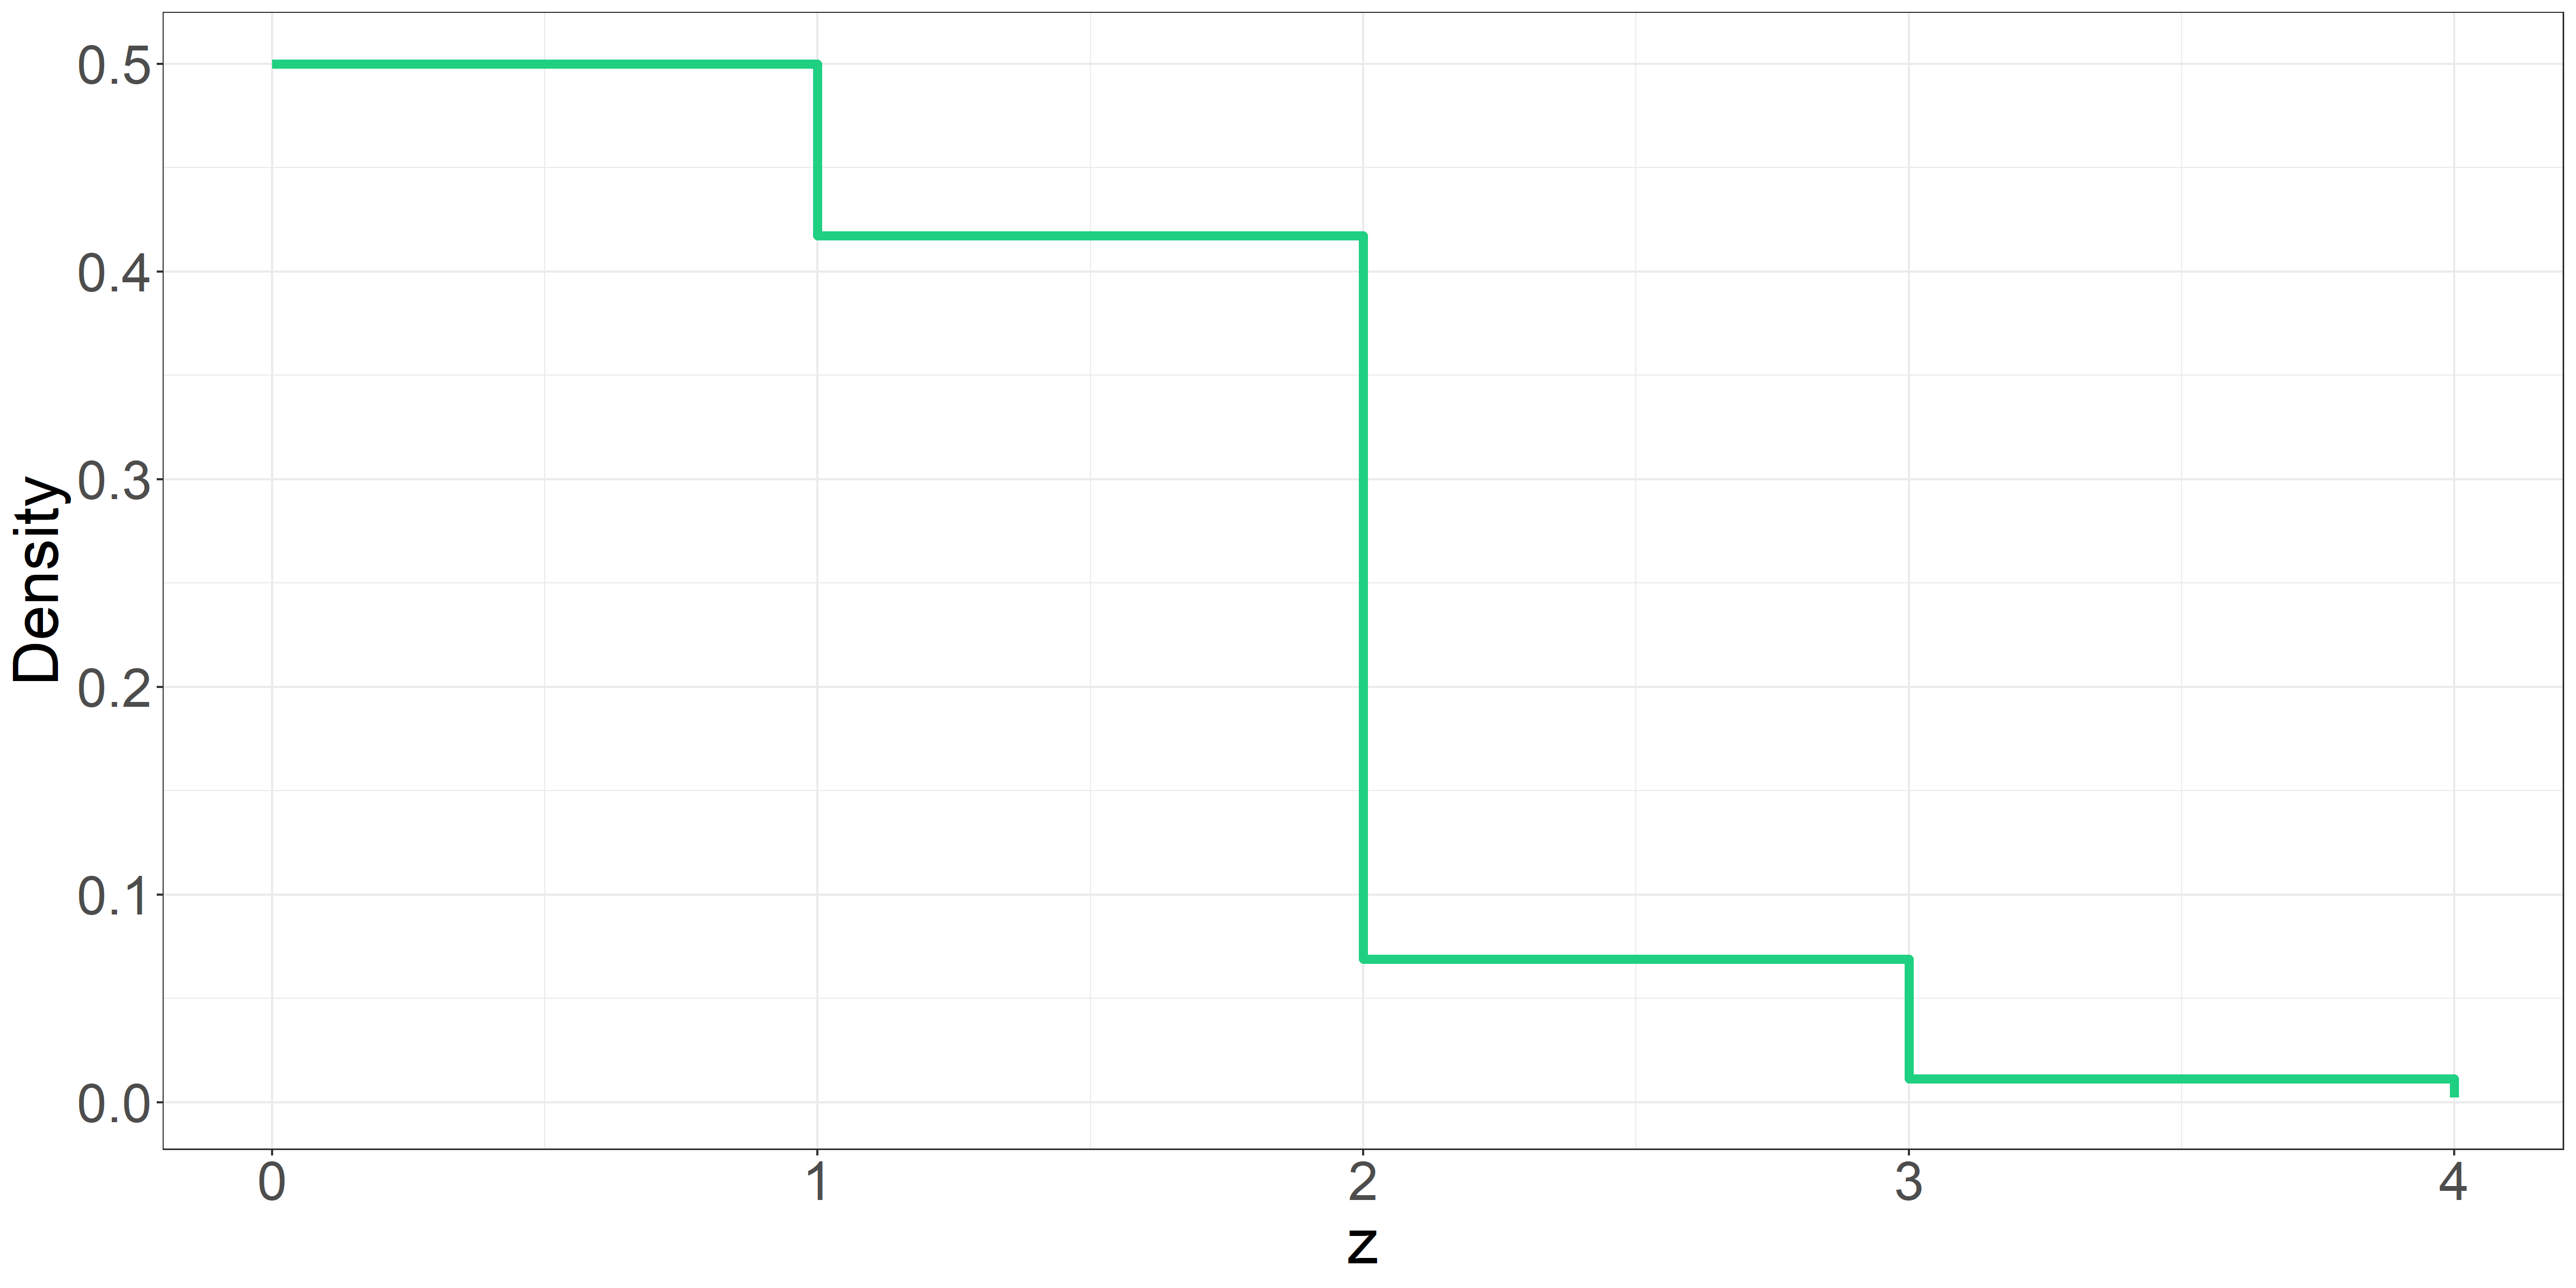
\includegraphics[width=1\linewidth]{../../figures/PDFLogNormal} \caption{Stairstep plot of the probability mass function for the discretized log-normal distribution with a mean of 0 and a standard deviation of 0.5, i.e.~\(Z \sim \lfloor \mathrm{LN}(0,0.5^2)\rfloor\).}\label{fig:PDFLogNormal}
\end{figure}

Typically, outbreak durations of 2-4 weeks are observed when values of \(k\) are in the range of 2-10. To simulate the outbreaks, the outbreak cases are added to the baseline count in week \(t_i+z_i\), where \(t_i\) represents the start time of the outbreak and \(z_i\) represents the number of weeks after the start of the outbreak. The start and end times of the outbreaks are recorded for evaluating the performance of the methods.

To simulate outbreaks, the following procedure is followed:

\begin{itemize} 
\item \textbf{Outbreaks in baseline weeks:} For each data series, four outbreaks are generated. The start time of each outbreak is randomly selected from the baseline weeks (weeks 313-575). The value of $k$ is sampled randomly with replacement from the set $\{2, 3, 5, 10\}$. It should be noted that different outbreaks are generated for each of the 2800 runs.
\item \textbf{Outbreaks in current weeks:} For each data series, one outbreak is generated. The start time of the outbreak is randomly chosen from the last 49 weeks (weeks 576-624). The value of $k$ is sampled randomly in the range of 1 to 10. Similar to the previous case, different outbreaks are generated for each of the 2800 runs.
\end{itemize}

One randomly chosen realization for scenario 8, 12, 13, and 20 are visualized in Figure \ref{fig:Realizations}.



\begin{figure}[H]
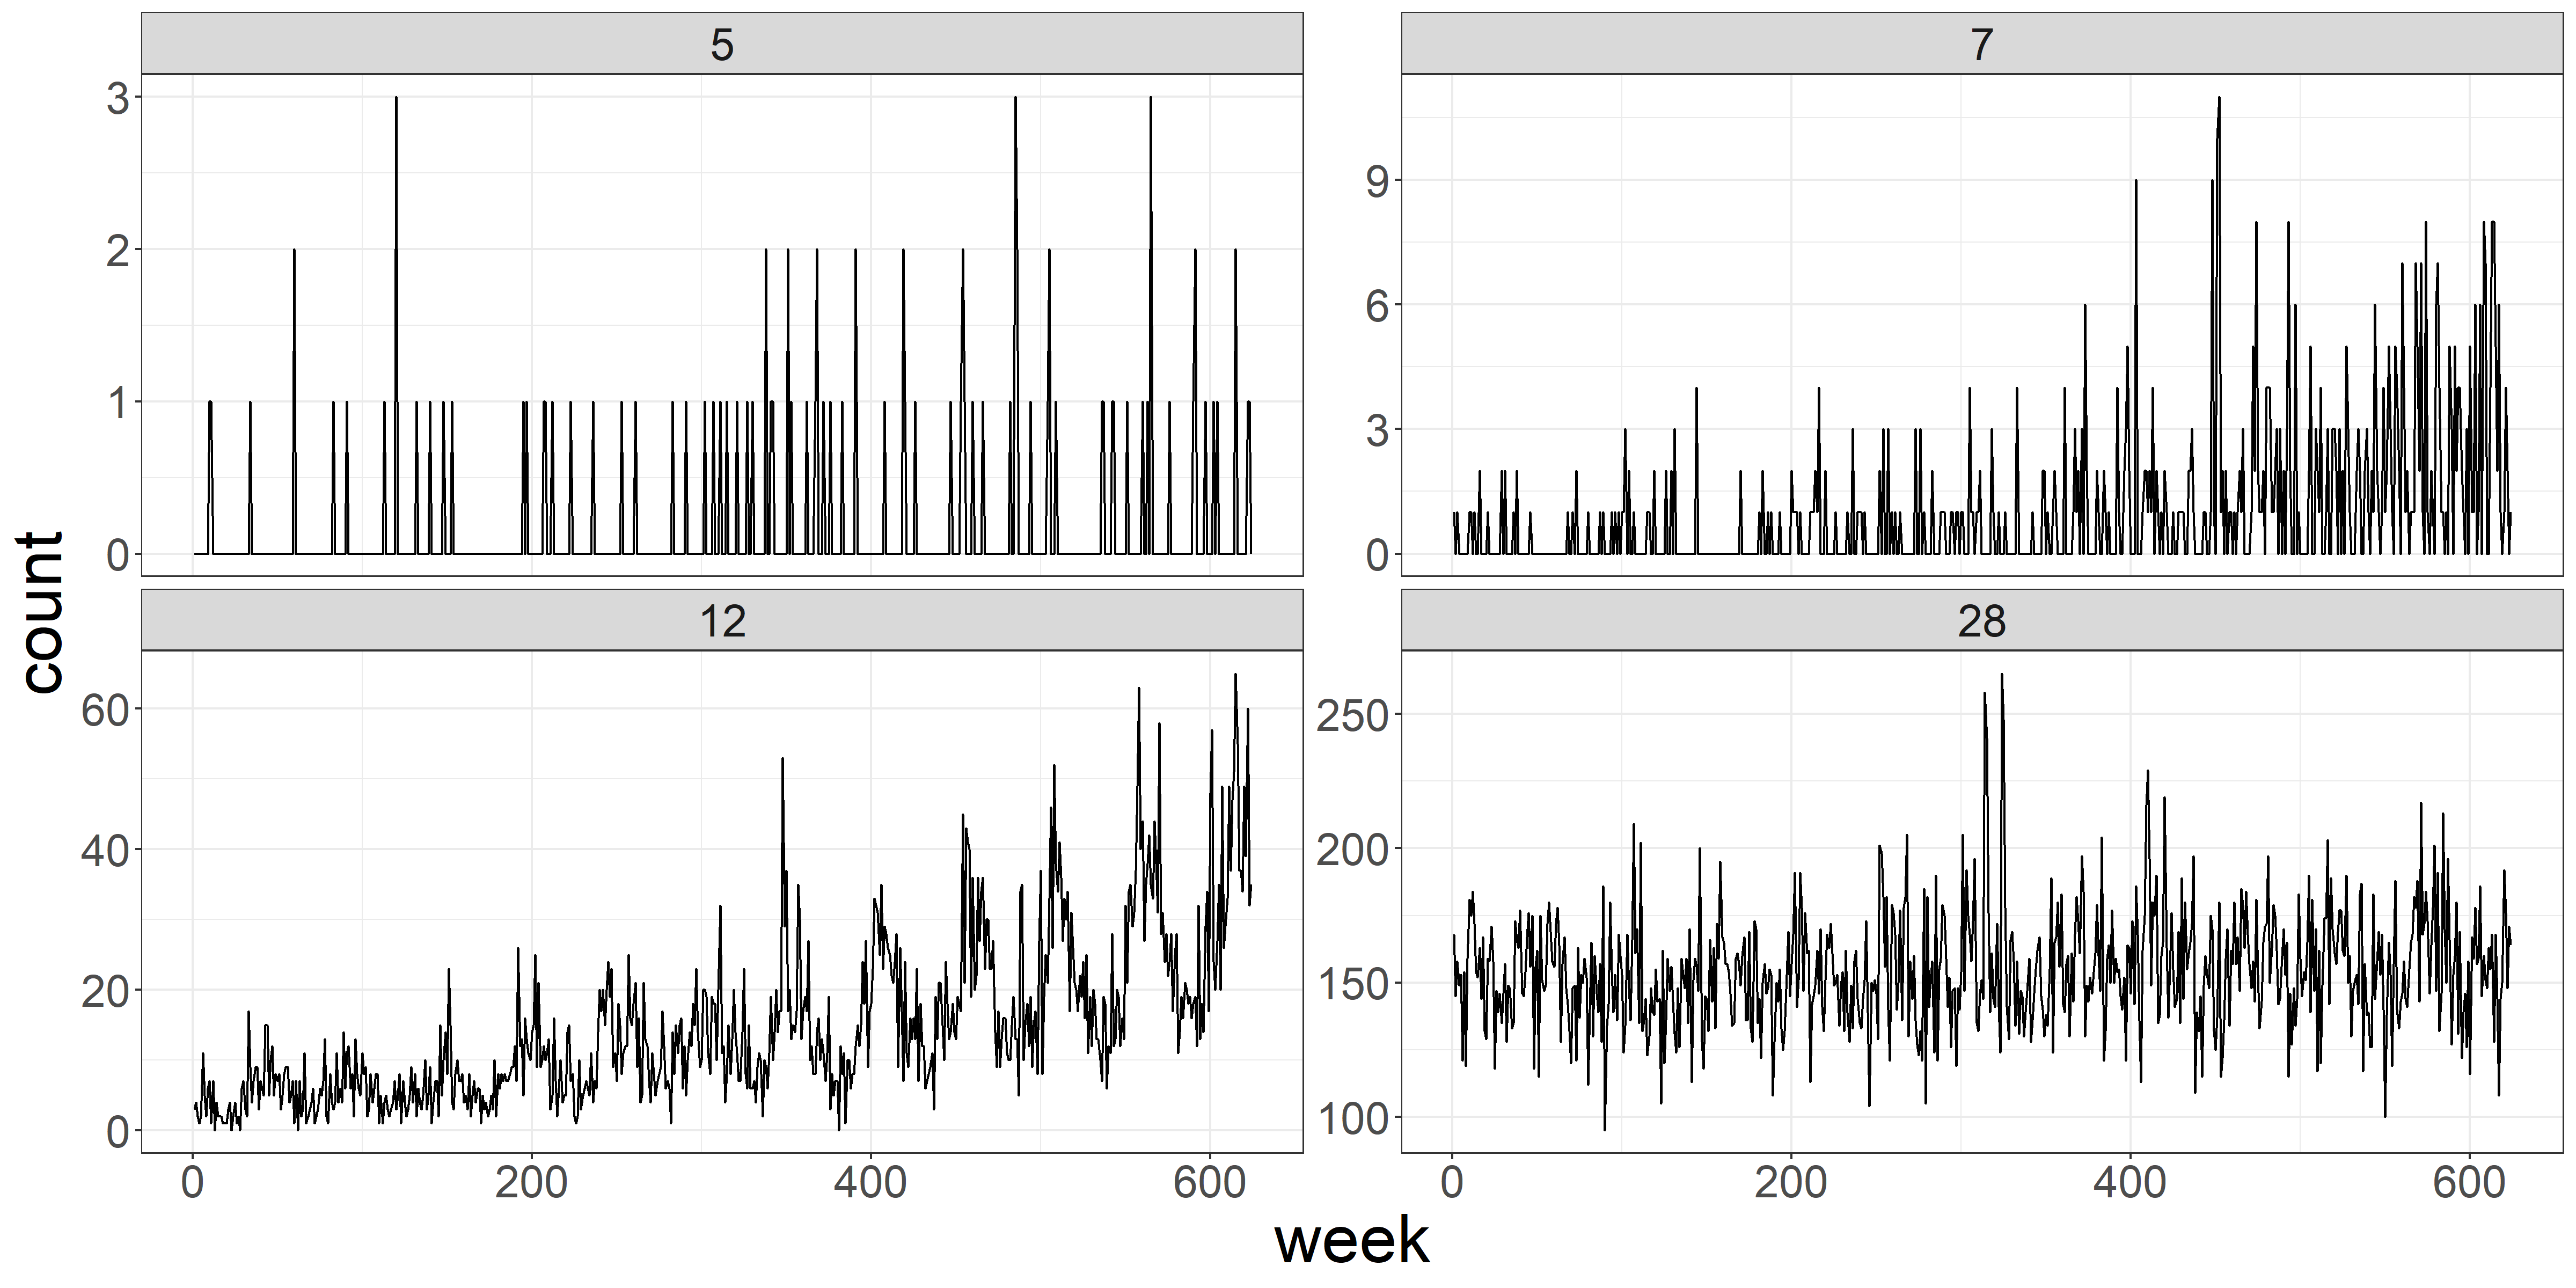
\includegraphics[width=1\linewidth]{../../figures/Realizations} \caption{Plots of one randomly chosen realization for scenario 8, 12, 13, and 20 (see Table \ref{tab:scenariosTbl}). During outbreaks (circles), outbreak cases are added to the baseline data. Four outbreaks are added during the baseline weeks and 1 outbreak is added during the test weeks. The results are based on the data obtained in the test weeks (grey area).}\label{fig:Realizations}
\end{figure}

Evidently, the scenarios vary in their epidemiological characteristics, such as seasonality, trend, and incidence.

\hypertarget{evaluation-measures}{%
\subsection{Evaluation measures}\label{evaluation-measures}}

To evaluate the performance of the outbreak detection system in the absence and presence of outbreaks, several measures are employed to assess its effectiveness. These measures are specifically designed to capture relevant quantities in the given context.

In the absence of outbreaks in the data, one of the primary measures used is the \emph{false positive rate} (FPR). This is calculated for each of the 28 scenarios, before the addition of the simulated outbreaks to the baseline data. The FPR is determined by calculating the proportion of the 49 weeks and 100 replicates in which the observed value exceeds the threshold in the absence of any simulated outbreaks.

Another measure is the \emph{probability of detection} (POD) of an outbreak. Likewise, this is calculated for each of the 28 scenarios, but this time it is in the presence of the simulated outbreaks. The algorithm is applied iteratively for the 49 current weeks, and an outbreak is considered detected if the observed value exceeds the threshold at least once within the start and end times of the outbreak. The POD of an outbreak is then determined as the proportion of outbreaks detected out of the 100 runs.

It is important to note that the FPR is a rate per week, while the POD is a rate per realization. These evaluation measures are chosen because they provide insights into the performance of the detection system on individual time series.

Finally, the \emph{diagnostic odds ratio} (DOR) is employed to measure the effectiveness of the outbreak detection methods. Using the terminology from a confusion matrix, the DOR is defined mathematically as:

\begin{equation}
\mathrm{DOR} = \frac{\mathrm{sensitivity} \times \mathrm{specificity}}{(1-\mathrm{sensitivity}) \times (1-\mathrm{specificity})}= \frac{\mathrm{TP}/\mathrm{FN}}{\mathrm{FP}/\mathrm{TN}}
\end{equation}

\hypertarget{results-of-the-simulation-study}{%
\section{Results of the simulation study}\label{results-of-the-simulation-study}}

\hypertarget{false-positive-rate}{%
\subsection{False positive rate}\label{false-positive-rate}}

In general, the method introduced by \citet{Farrington_1996} exhibits relatively higher FPRs compared to the other methods. This outcome is not surprising since the Farrington method is known to be overly sensitive, making it more prone to producing false alarms. This sensitivity concern was further recognized by \citet{Noufaily_2013}, prompting the development of a new and improved method. Moreover, this observation is consistent with the results of the simulation study conducted in this article, as illustrated in Figure \ref{fig:FPRalphamethodsmedian}, which presents the median FPRs obtained across the 100 replications in each of the 28 simulated scenarios, demonstrating the methods performance under varying significance levels for the threshold calculation. For boxplots of the FPRs, refer to Figure \ref{fig:FPRalphamethods}.



\begin{figure}[H]
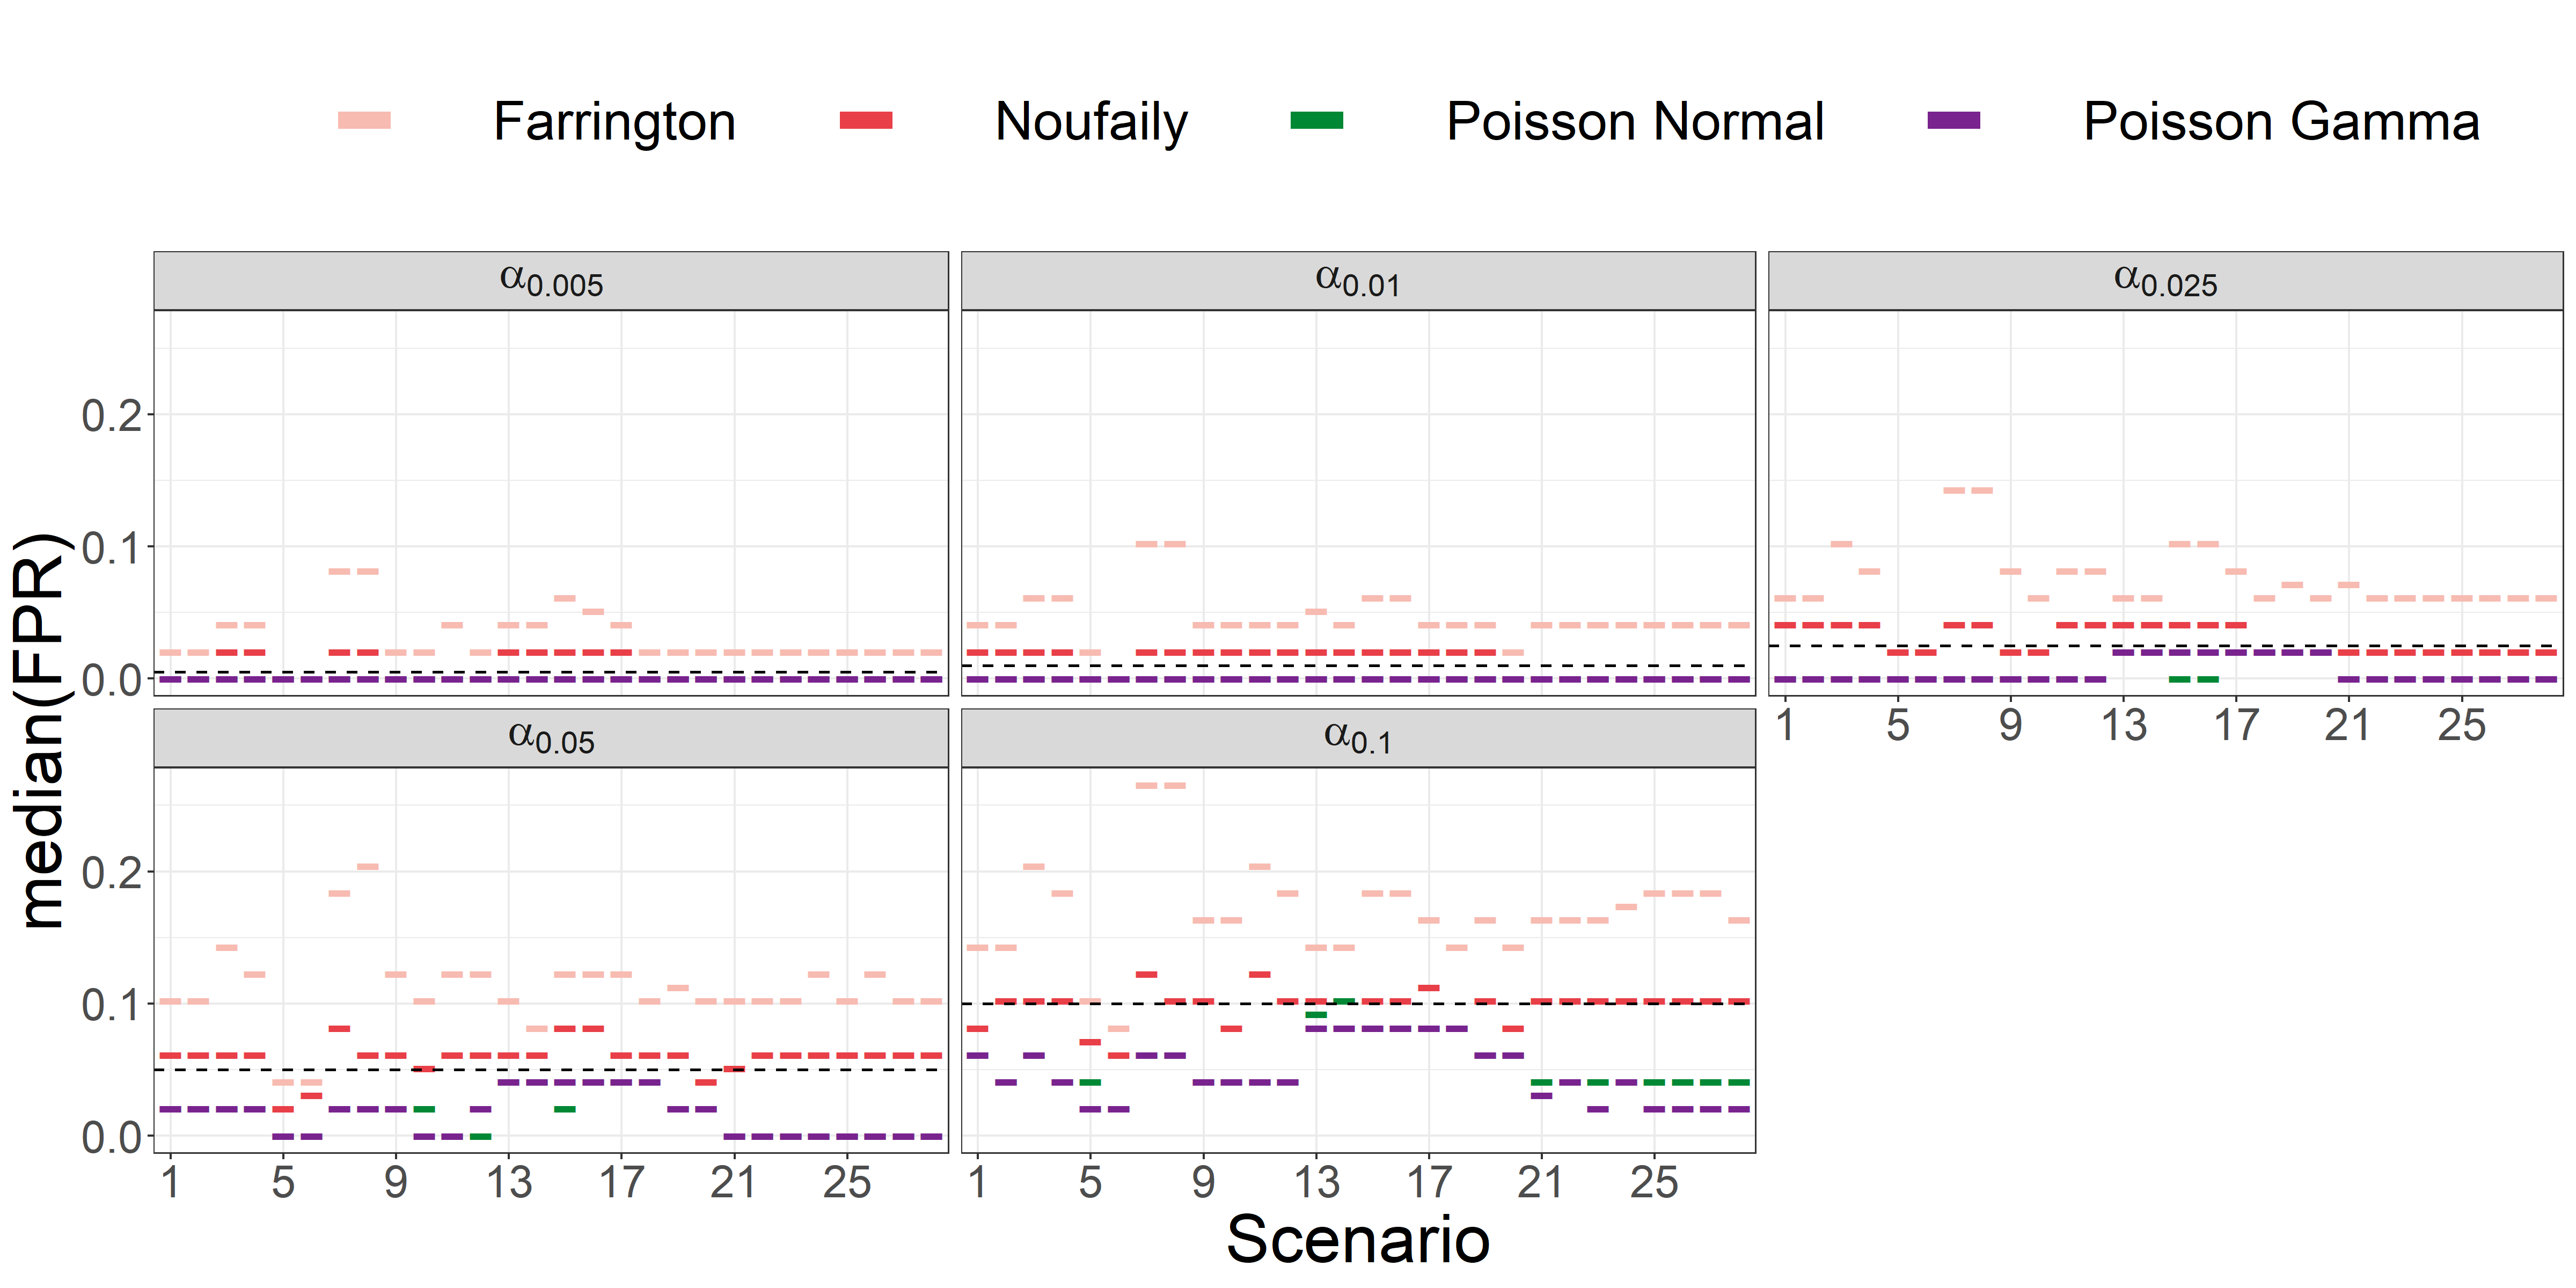
\includegraphics[width=1\linewidth]{../../figures/FPR_alpha_methods_median} \caption{Median FPRs obtained across the 100 replications in each of the 28 scenarios by employing each of the different methods with varying significance levels, \(\alpha\). The dashed lines represents the nominal values.}\label{fig:FPRalphamethodsmedian}
\end{figure}

Inspecting the figure, it is clear that the Farrington method tends to underperform in scenario 7 and 8, which are scenarios characterized by a steep trend. The Noufaily method resolves this issue, generally outperforming the Farrington method. Moreover, the novel methods consistently outperforms the other methods. However, it is interesting to note that scenario 13 trough 20 prove to be particularly problematic for the novel methods. A closer look reveals that these scenarios are characterized by a high overdispersion parameter, indicating increased variability in the data. Lastly, it is crucial to acknowledge that the median FPRs for the novel methods remain within nominal values.

\hypertarget{probability-of-detection}{%
\subsection{Probability of detection}\label{probability-of-detection}}

As anticipated, the POD of an outbreak increases with the size of \(k\). Intuitively, when the outbreak size \(v\) is larger, it becomes more likely to be detected by the outbreak detection algorithms. In the simulation study presented in this article, the Farrington method demonstrates excellent performance in terms of POD, closely followed by the Noufaily method. The high performance of the Farrington method can be attributed to its sensitivity in detecting outbreaks.

Moreover, it is crucial to emphasize the importance of careful parametrization for the novel methods. Unlike the established methods, the novel approaches are inherently less sensitive, necessitating a higher significance level, \(\alpha\), for the threshold calculations. This is illustrated in Figure \ref{fig:PODalphamethodsmedian}, which depicts the median POD for different sizes of \(k\) across the 100 replications for each of the 28 scenarios. Refer to \ref{fig:PODalphamethods}, to see the variability in the POD for each scenario together with the median POD.



\begin{figure}[H]
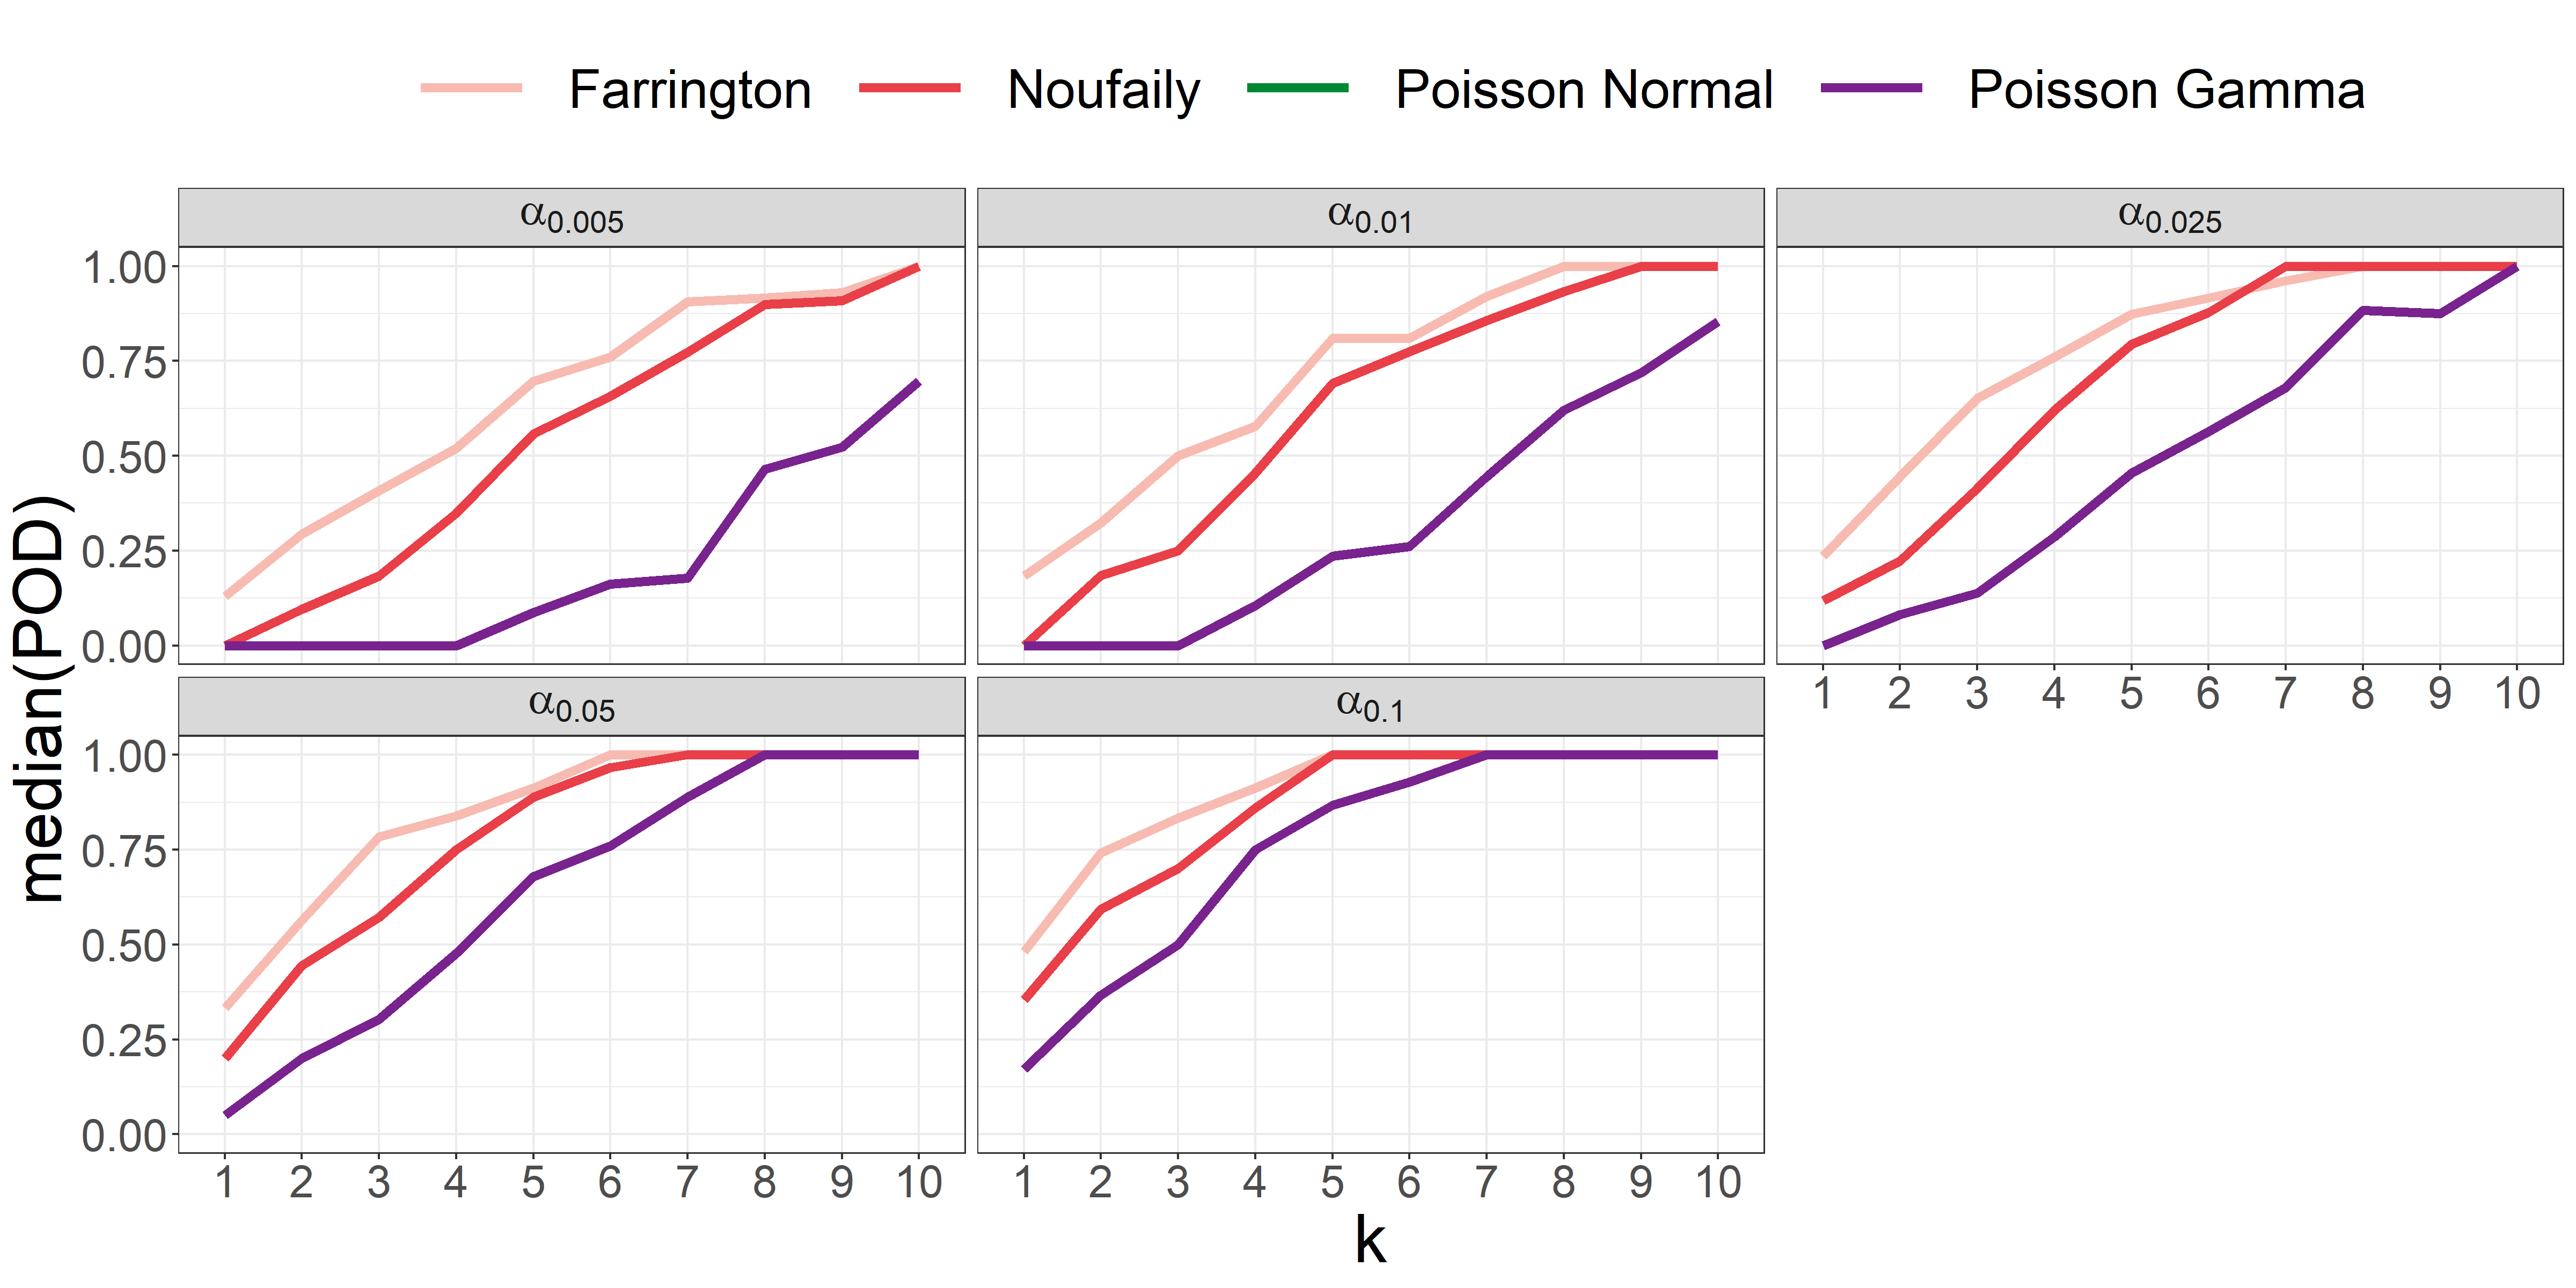
\includegraphics[width=1\linewidth]{../../figures/POD_alpha_methods_median} \caption{Median POD of an outbreak of a random size \(v\) drawn from a Poisson distribution with mean equal to \(k\) times the standard deviations of the baseline data for different values of \(\alpha\). The x-axis shows increasing values of \(k\), while the y-axis shows the median POD across the 100 replications for each of the 28 scenarios.}\label{fig:PODalphamethodsmedian}
\end{figure}

It is important to bear in mind that an outbreak of size \(v\) is randomly distributed in time according to a discretized log-normal distribution with a mean of \(0\) and a standard deviation of \(0.5\), denoted as \(Z \sim \lfloor \mathrm{LN}(0,0.5^2)\rfloor\). The probability mass function of \(Z\) is shown in Figure \ref{fig:PDFLogNormal}. From the figure, it can be observed that \(50\%\) of the outbreak cases are added to the same week as the outbreak starts, \(42\%\) are added to the following week, and only \(7\%\) are added two weeks after the start. Therefore, the simulated outbreak cases are not observed in a single week only but rather in several concurrent weeks.

Consequently, an outbreak of size \(v\) generated from a Poisson distribution with a mean equal to \(k\) times the standard deviation of the baseline series is perceived to be relatively smaller than initially perceived in the simulation setup. For example, an outbreak of size \(k=4\) times the standard deviation may only be perceived as an outbreak signal of size \(2\) times the standard deviation in an individual week.

\hypertarget{diagnostic-odds-ratio}{%
\subsection{Diagnostic odds ratio}\label{diagnostic-odds-ratio}}

When evaluating the performance of an outbreak detection method, it is crucial to consider its relevance in real-world implementations. Historically, both of the established methods have been associated with generating an excessive number of false alarms, placing a burden on epidemiologists who must undertake tedious verification tasks. Hence, the DOR is chosen as a metric to gauge the effectiveness of the outbreak detection methods.

Upon inspecting Figure \ref{fig:logDORalpha}, it becomes apparent that the novel methods outperform the established ones concerning the DOR. The DOR consistently favors the novel methods across various sizes of \(k\). Moreover, it can be seen that for medium-sized outbreaks, \(4\leq k \leq 6\), a significance level of \(\alpha=0.025\) maximizes the DOR for the novel methods, while for large outbreaks, \(k>6\), a significance level of \(\alpha\leq 0.01\) is favorable.



\begin{figure}[H]
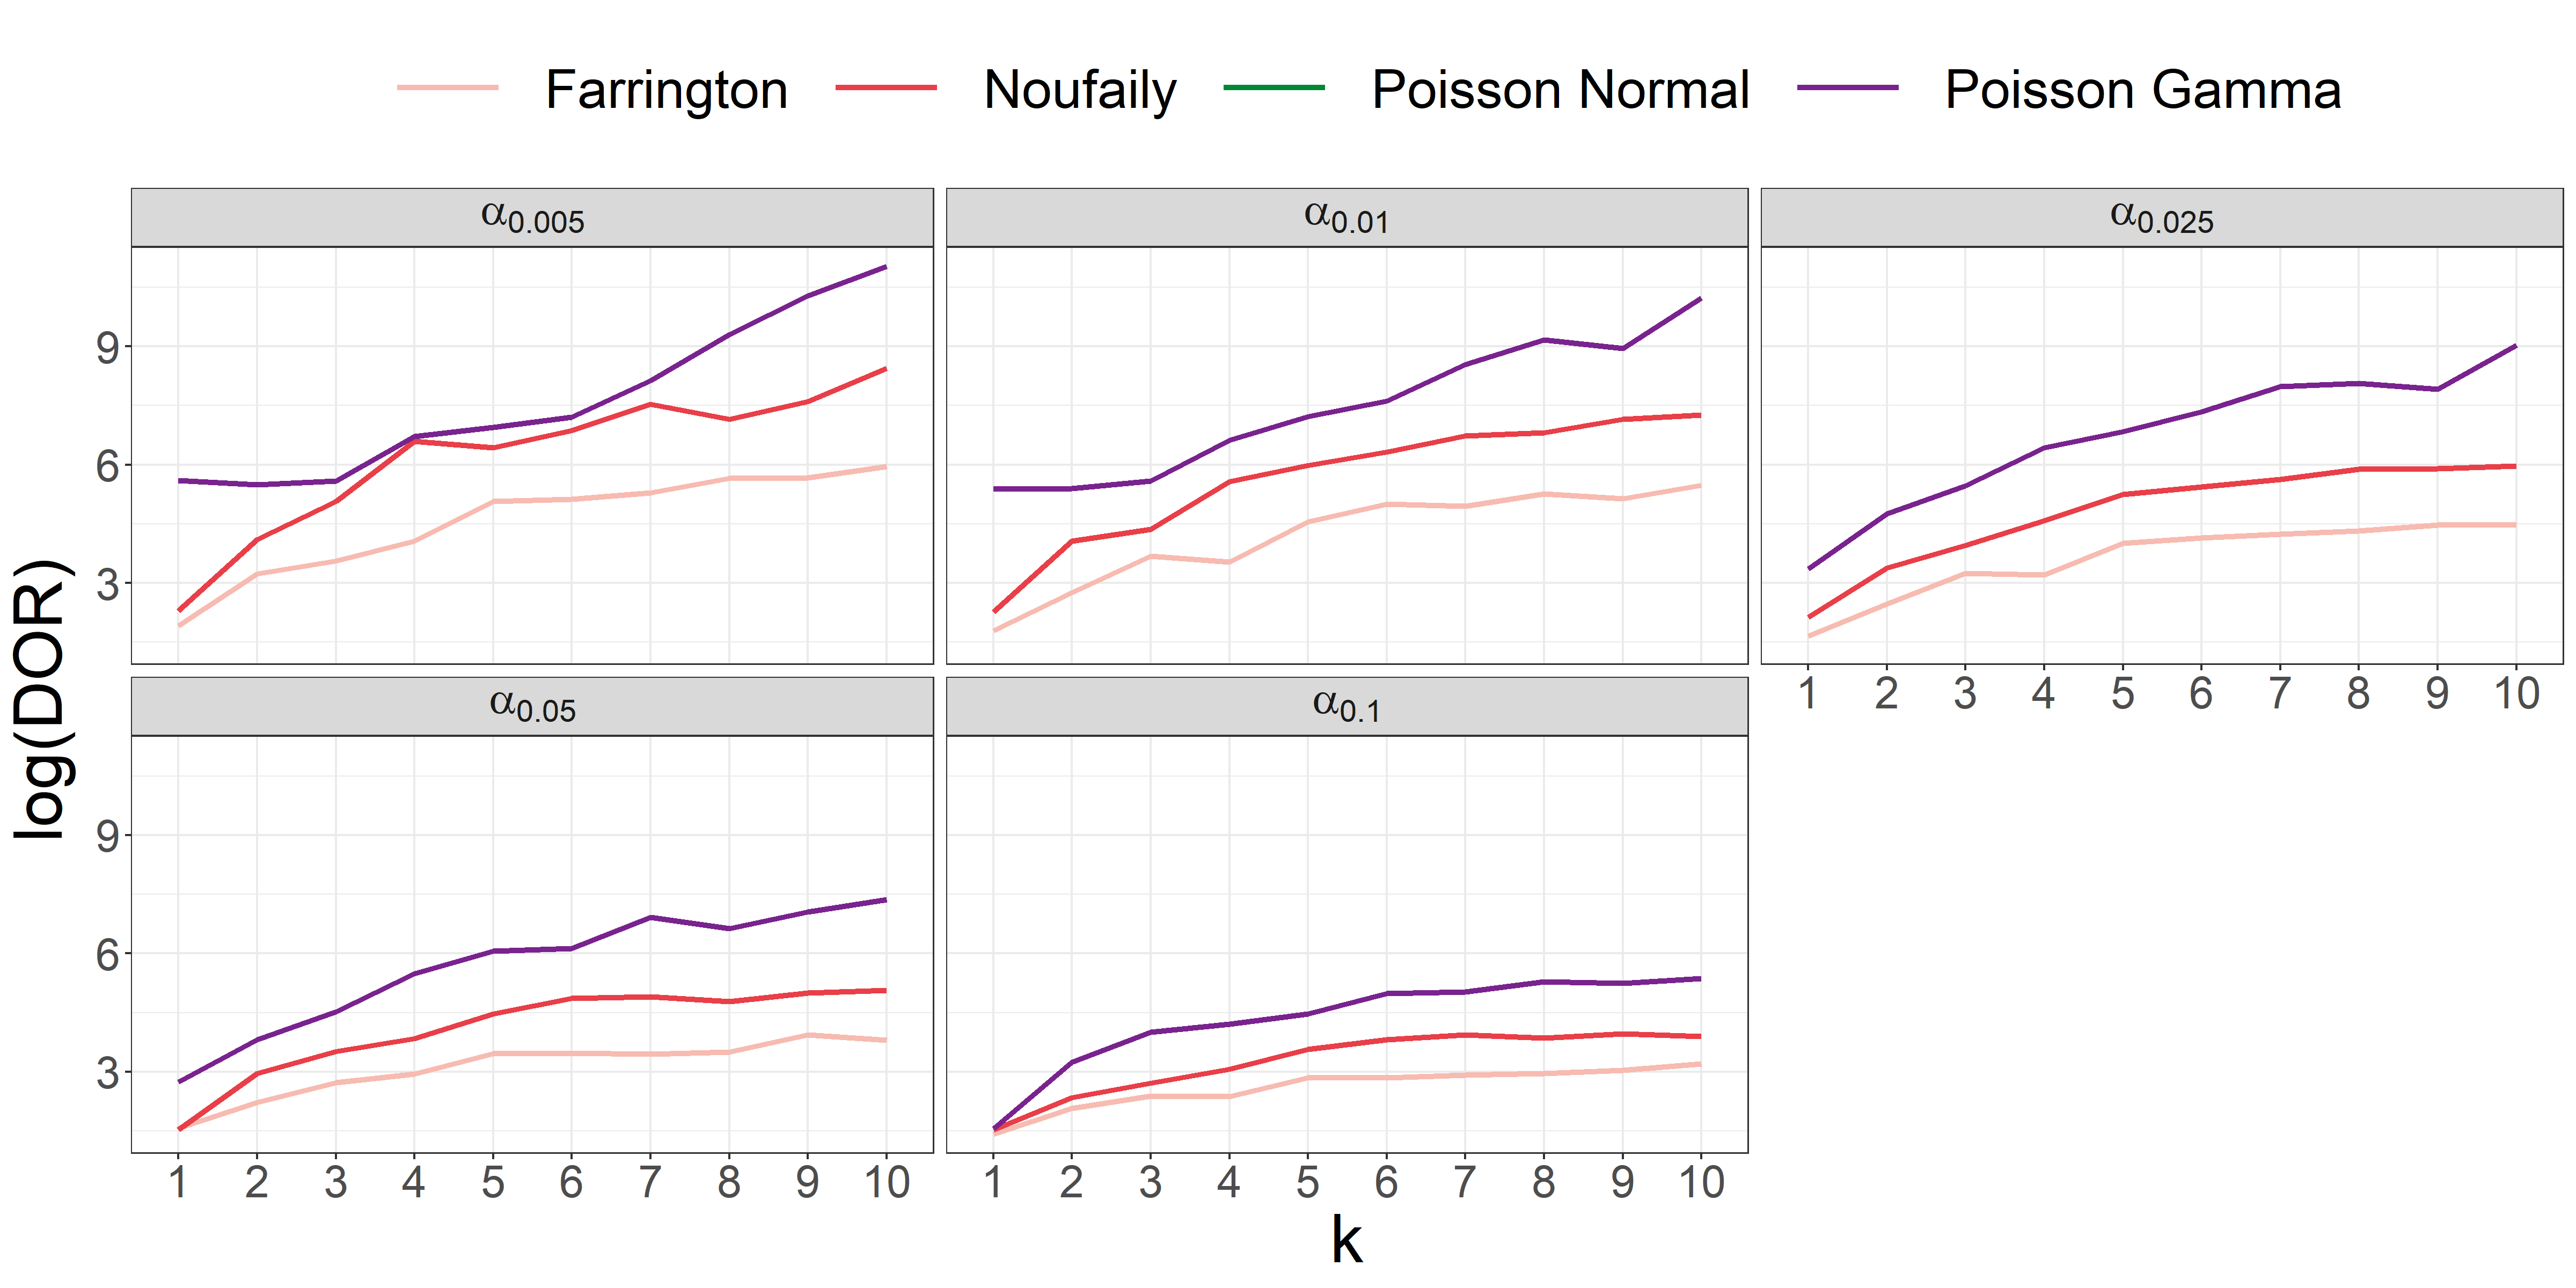
\includegraphics[width=1\linewidth]{../../figures/logDOR_alpha} \caption{Logarithmic DOR of an outbreak of a random size \(v\) drawn from a Poisson distribution with mean equal to \(k\) times the standard deviations of the baseline data for different values of \(\alpha\). The x-axis shows increasing values of \(k\), while the y-axis shows the logarithmic DOR across the 100 replications for each of the 28 scenarios.}\label{fig:logDORalpha}
\end{figure}

\hypertarget{evaluations-on-data}{%
\section{Evaluations on data}\label{evaluations-on-data}}

In order to evaluate the performance of the statistical outbreak detection methods considered in this article, a real-life case study of shiga toxin-producing Escherichia coli (STEC) is investigated.

\hypertarget{epidemiological-background-and-notable-outbreaks-of-shiga-toxin-producing-escherichia-coli}{%
\subsection{\texorpdfstring{Epidemiological background and notable outbreaks of shiga toxin-producing \emph{Escherichia coli}}{Epidemiological background and notable outbreaks of shiga toxin-producing Escherichia coli}}\label{epidemiological-background-and-notable-outbreaks-of-shiga-toxin-producing-escherichia-coli}}

STEC primarily spreads through contaminated food. Less common sources of infection include contaminated drinking and bathing water, as well as direct of indirect contact with infected animals. Cattle and other ruminants are primary reservoirs for STEC serotypes that are frequently associated with human disease \citep{Menge_2020}. Hemolytic uremic syndrome (HUS) is a severe complication that, in some cases, particularly in children, can develop following an infection with STEC.

One of the earliest documented STEC outbreaks occured in 2007, involving 18 laboratory confirmed cases over a six-week period. Investigations indicated a specific brand of organic beef sausage as the likely source of infection.

In September to October 2012, a STEC outbreak with a high risk of HUS was observed. Thirteen cases were diagnosed, with eight individuals developing HUS. Epidemiological investigations suggested that ground beef was the vehicle of the outbreak \citep[\citet{Helwigh_2013}]{Soborg_2013}.

More recent outbreaks include a 38-case outbreak from September to November 2018, with a suspected association with beef sausage as the source of infection \citep{Helwigh_2019}. Additionally, there were two unresolved outbreaks with 11 and 14 cases occurring from May to July 2019 and from December 2021 to January 2022, respectively. The latter outbreak included three cases of HUS

Common for the above outbreaks are, that they are well-documented outbreak investigated by Statens Serum Institut (SSI).

\hypertarget{the-data}{%
\subsection{The data}\label{the-data}}

The data set is publicly available and can be accessed at \url{https://statistik.ssi.dk/}. It comprises monthly counts of Danish STEC cases, denoted as \(y_{it}\). For the purpose of this article, the cases are divided into six functional age groups, namely: below 1 year, between 1-4 years, 5-14 years, 15-24 years, 25-64 years, and 65 years and above. Thus the index \(i=1,\dots,6\) represents the six age groups and \(t=1,\dots,T\) represents the time period of \(T=180\) months starting in 2008. The distribution of cases in these age groups is visualized in a stacked bar graph in Figure \ref{fig:STEC}.



\begin{figure}[H]
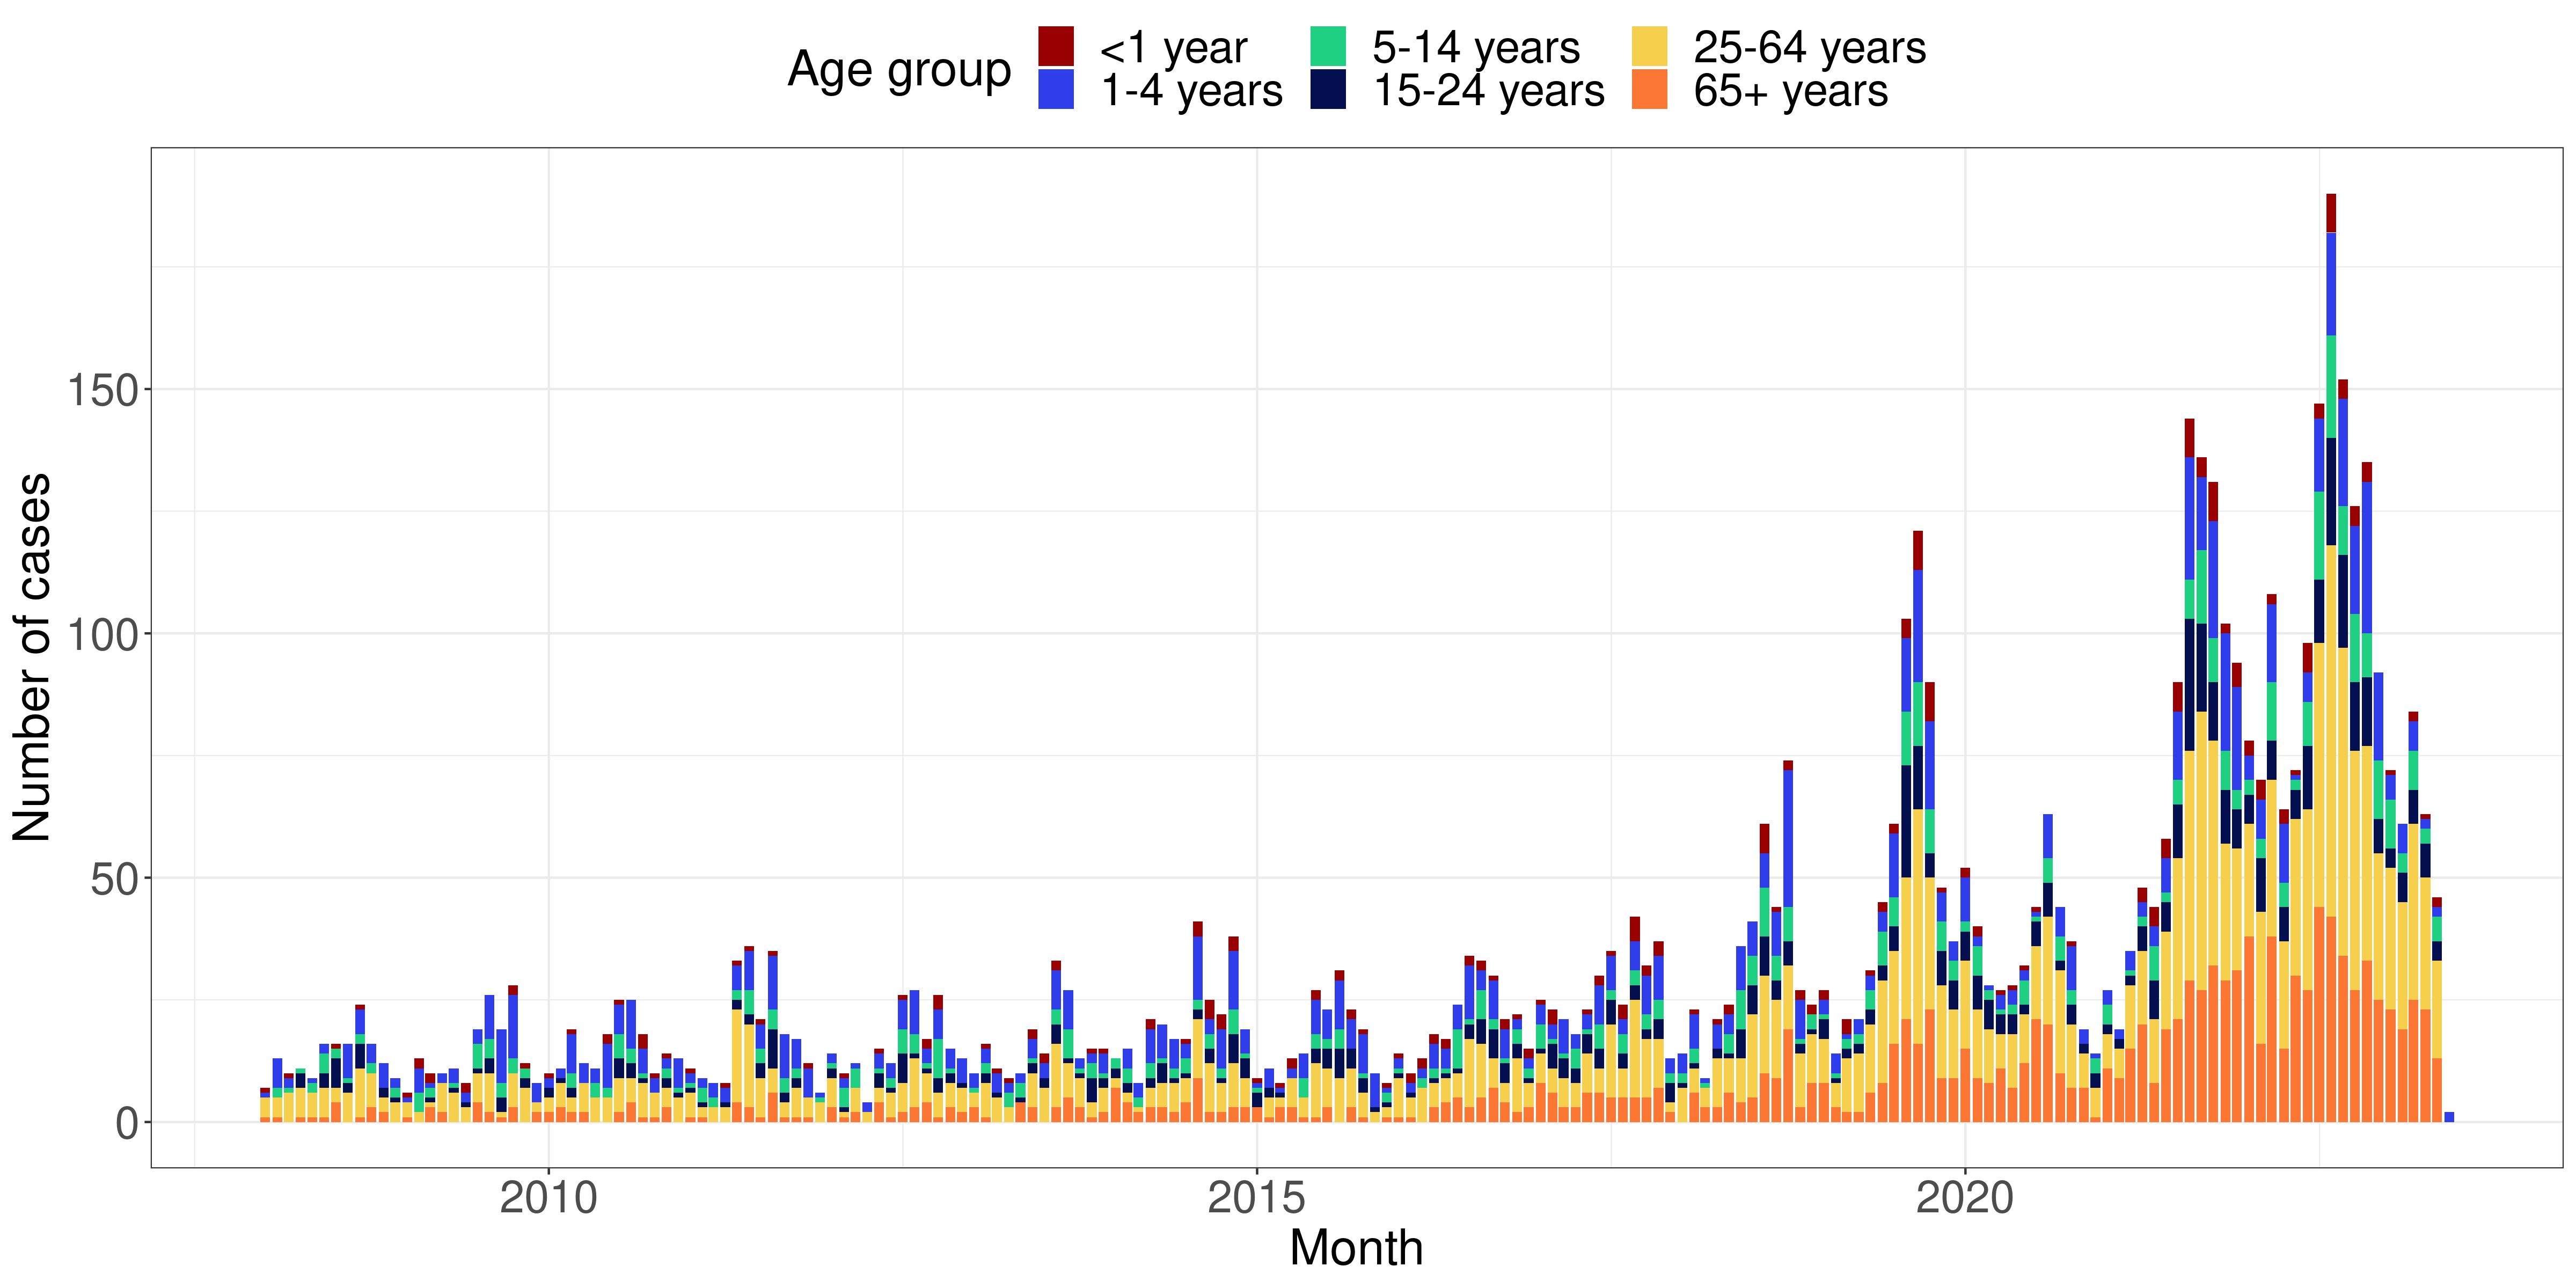
\includegraphics[width=1\linewidth]{../../figures/STEC_long_plot} \caption{A stacked bar graph illustrating the number of monthly STEC cases observed in the period from 2008 to 2022 for the six age groups.}\label{fig:STEC}
\end{figure}

In the figure, a notable increase in the amplitude of the seasonal variation is observed starting from 2018, with incidences doubling compared to preceding years. At a first glance, this increase in the incidences might be recognized as a serious, reoccurring outbreak of the disease, but a more reasonable explanation can be found. Up to 2018, most departments of clinical microbiology used culture based methods as a diagnostic test for bacterial pathogens and the process of changing the test method to polymerase chain reaction (PCR) methods was ongoing \citep{Svendsen_2023}. In general, the PCR method resulted in higher incidences compared to the other diagnostic methods.

\hypertarget{applying-the-detection-methods}{%
\subsection{Applying the detection methods}\label{applying-the-detection-methods}}

To investigate and compare the performance of the outbreak detection methods, the method by \citet{Farrington_1996} and the subsequently improved method by \citet{Noufaily_2013} are explored. The methods are controlled using specific \texttt{control} arguments. Here, a period of \(b=3\) years and a window half-width of \(w=2\) is chosen for the reference data. Consequently, the number of baseline months used to calculate the thresholds are based on a total of \(n^{m}=15\) months. Also, the threshold calculation is based on a significance level of \(\alpha=0.005\). This significance level is chosen based on the simulation results in this article, to effectively control the number of false alarms generated by the established methods, and because it was shown that this level maximizes the DOR.

For the novel method, an observation is classified as an outbreak if the one-step ahead random effect \(u_{it_1}\) for the specific age group exceeds the upper bound \(U_{t_0}\). In this case study, the upper bound is determined as the \(97.5\%\) quantile of the distribution of random effects obtained from the second stage model, as it was shown that this value maximizes the DOR for medium-sized outbreaks. Moreover, the disease intensity, \(\lambda_{it}\), is modeled as follows:

\begin{equation}
  \log{\lambda_{it}}=\beta(ageGroup_i) + \beta_{trend} t + \sin\big(\frac{2\pi\cdot\tau_t}{12}\big) + \cos \big(\frac{2\pi\cdot\tau_t}{12}\big) + \log(n_{it})
\end{equation}

Here \(\beta(ageGroup_i)\) represents the fixed effect specific to the age group \(i\) on the outbreak intensity, \(\beta_{trend}\) quantifies the rate of change in the intensity over time, \(\beta_{\sin}\) and \(\beta_{\cos}\) capture the effect of the seasonal pattern, and \(\log(n_{it})\) acts as an offset, accounting for the population size at time \(t\) for age group \(i\). These parameters are estimated using a rolling window of width \(k=36\) months.

\hypertarget{performance-of-statistical-outbreak-detection-methods}{%
\subsection{Performance of statistical outbreak detection methods}\label{performance-of-statistical-outbreak-detection-methods}}

The primary challenge in evaluating methods for automated and early detection of disease outbreaks lies in the difficulty to precisely defining what constitutes an outbreak. In the case study presented in this article, an outbreak is defined as an event that is officially investigated and documented by SSI. However, this definition lacks standardization and reproducibility, relying heavily on individual epidemiologists' perceptions of an outbreak and their capacity to allocate resources for investigation and documentation. Consequently, in the absence of a universally accepted and standardized definition of outbreaks, the documented investigations conducted by epidemiologists at SSI have been utilized for evaluation purposes.

Figure \ref{fig:CompareAlarms} demonstrates that the established methods, especially the Farrington method, raise a higher number of alarms in comparison to the novel methods.



\begin{figure}[H]
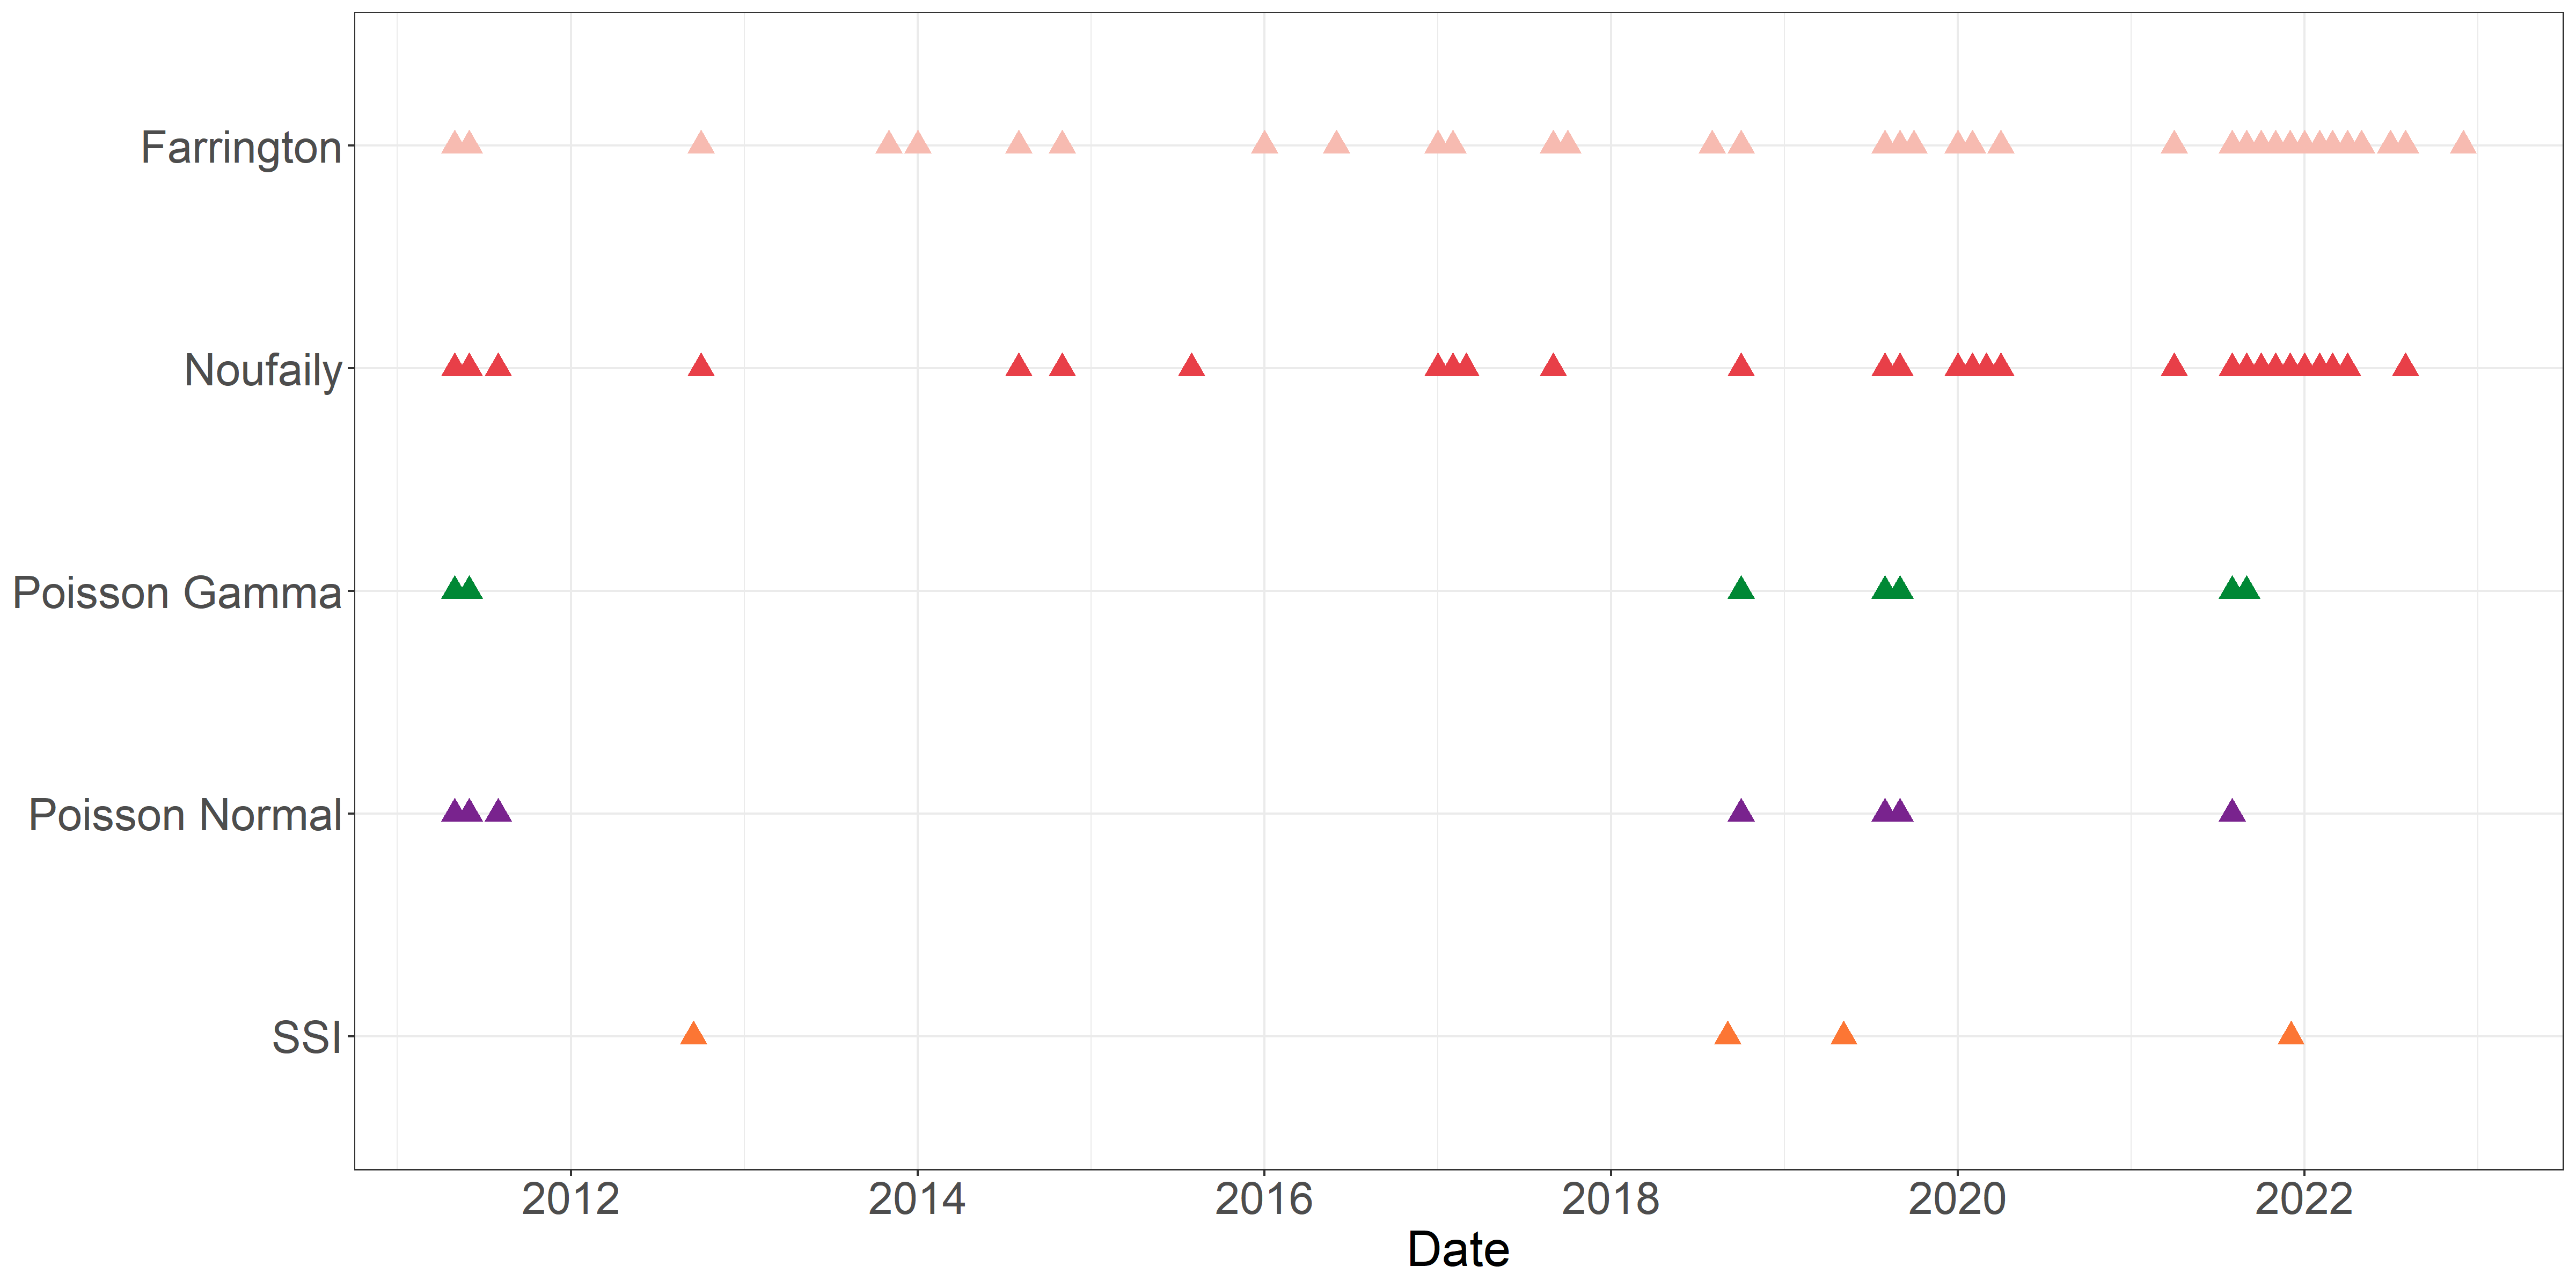
\includegraphics[width=1\linewidth]{../../figures/Compare_alarms_STEC_article} \caption{Alarm plot displaying alarms for the STEC time series using the four different outbreak detection methods, along with well-documented outbreaks investigated by SSI.}\label{fig:CompareAlarms}
\end{figure}

\hypertarget{discussion}{%
\section{Discussion}\label{discussion}}

The field of automated disease outbreak detection has witnessed substantial advancements in recent years, marked by the development of sophisticated statistical methods and the utilization of computerized databases. These advancements hold tremendous potential in supplementing epidemiologists, aiding them in efficiently prioritizing efforts and allocating resources for more targeted outbreak management strategies. However, an emerging concern in the field is the phenomenon known as ``alarm fatigue'' and its implications for statistical outbreak detection.

Alarm fatigue refers to the desensitization and decreased responsiveness that can occur when epidemiologists are exposed to frequent or excessive alarms from outbreak detection methods. Specifically, the method introduced by \citet{Farrington_1996} is known for its occasional lack of specificity, leading to false alarms that can overwhelm epidemiologists with verification tasks. Consequently, its usefulness and practicality in real-world settings are undermined. In an effort to address the number of false alarms, the subsequently improved method by \citet{Noufaily_2013} was introduced. While it was found that this method greatly reduced the number of alarms while maintaining good overall performance in detecting outbreaks, it has been unable to establish itself as a reliable method.

An outbreak detection algorithm that can effectively control the number of false alarms, while still maintaining the power to detect genuine outbreaks, is increasingly high demand. This article demonstrates that the proposed novel method has immense potential as a candidate tool for outbreak detection. It considerably reduces the number of alarms generated compared to the Farrington and Noufaily methods while still maintaining the ability to generate alarms that coincide in time with simulated outbreaks. This finding is underscored by the fact that the novel method consistently outperformed the established methods when measure on the \emph{diagnostic odds ratio}. Furthermore, the novel method allows for covariate incorporation, distinguishing it from both the Farrington and Noufaily methods. These finding highlight the potential of hierarchical models as a framework for outbreak detection in general.

\hypertarget{conclusion}{%
\section{Conclusion}\label{conclusion}}

Lorem ipsum dolor sit amet, consectetur adipiscing elit, sed do eiusmod tempor incididunt ut labore et dolore magna aliqua. Ut enim ad minim veniam, quis nostrud exercitation ullamco laboris nisi ut aliquip ex ea commodo consequat. Duis aute irure dolor in reprehenderit in voluptate velit esse cillum dolore eu fugiat nulla pariatur. Excepteur sint occaecat cupidatat non proident, sunt in culpa qui officia deserunt mollit anim id est laborum.

\newpage

\appendix

\hypertarget{additional-figures}{%
\section{Additional figures}\label{additional-figures}}

\hypertarget{false-positive-rate-1}{%
\subsection{False positive rate}\label{false-positive-rate-1}}



\begin{figure}[H]
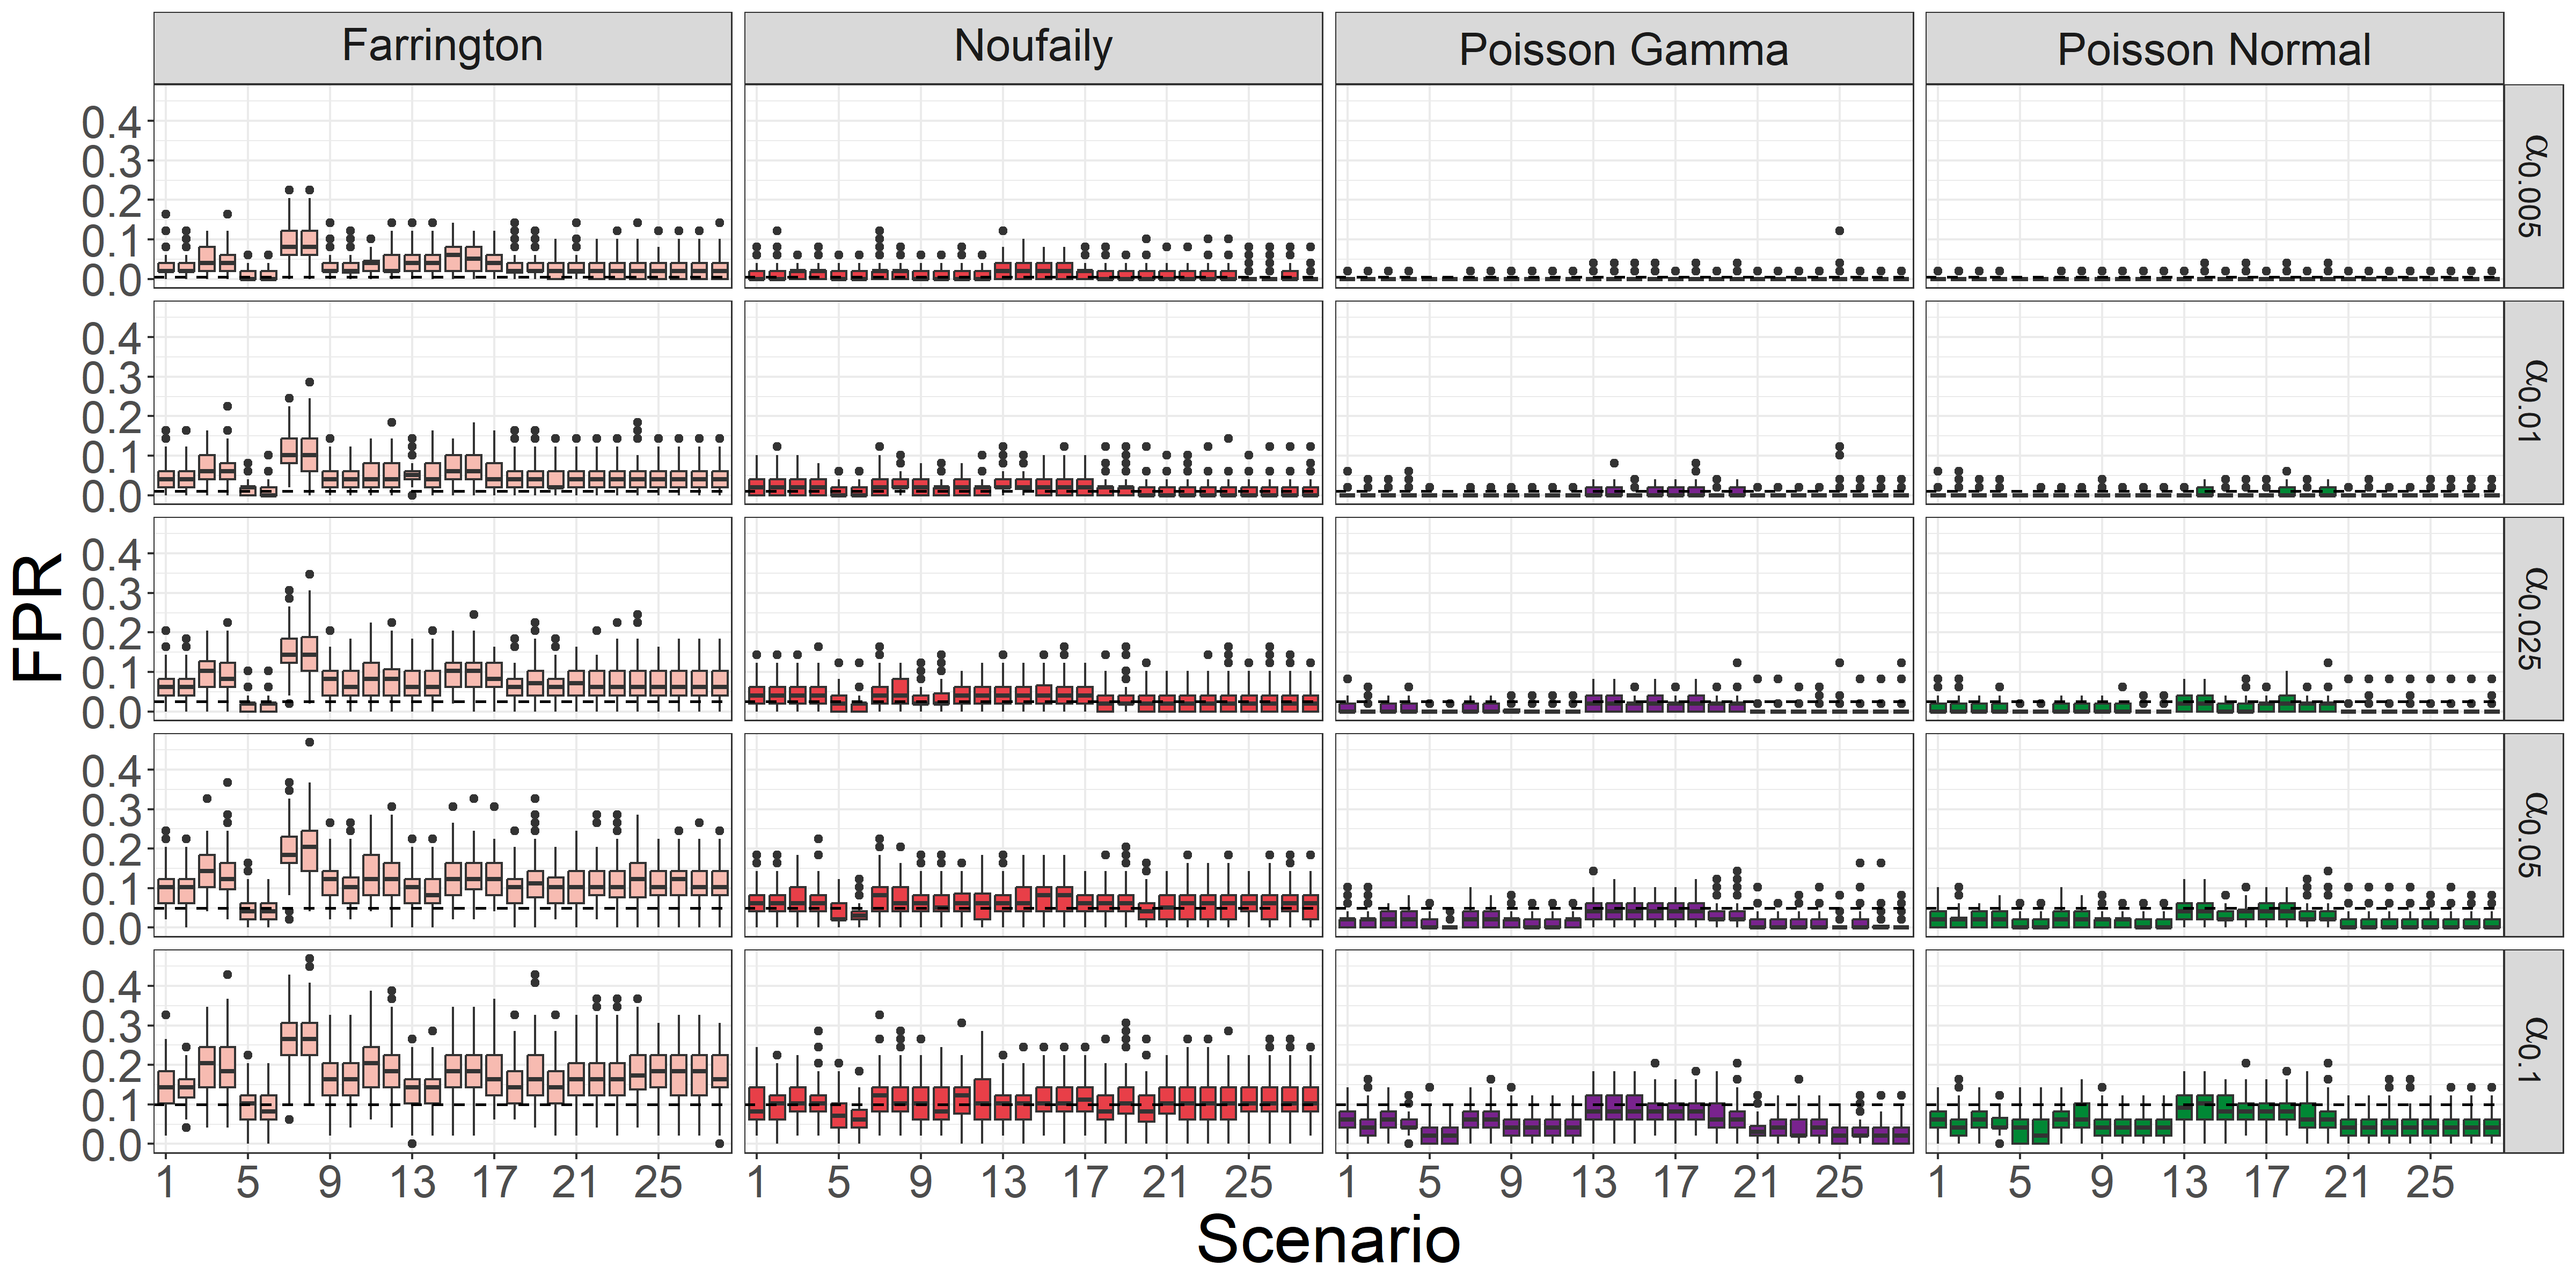
\includegraphics[width=1\linewidth]{../../figures/FPR_alpha_methods} \caption{FPRs obtained across the 100 replications in each of the 28 scenarios by employing each of the different methods with varying significance levels, \(\alpha\). The dashed lines represents the nominal values.}\label{fig:FPRalphamethods}
\end{figure}

\hypertarget{probability-of-detection-1}{%
\subsection{Probability of detection}\label{probability-of-detection-1}}



\begin{figure}[H]
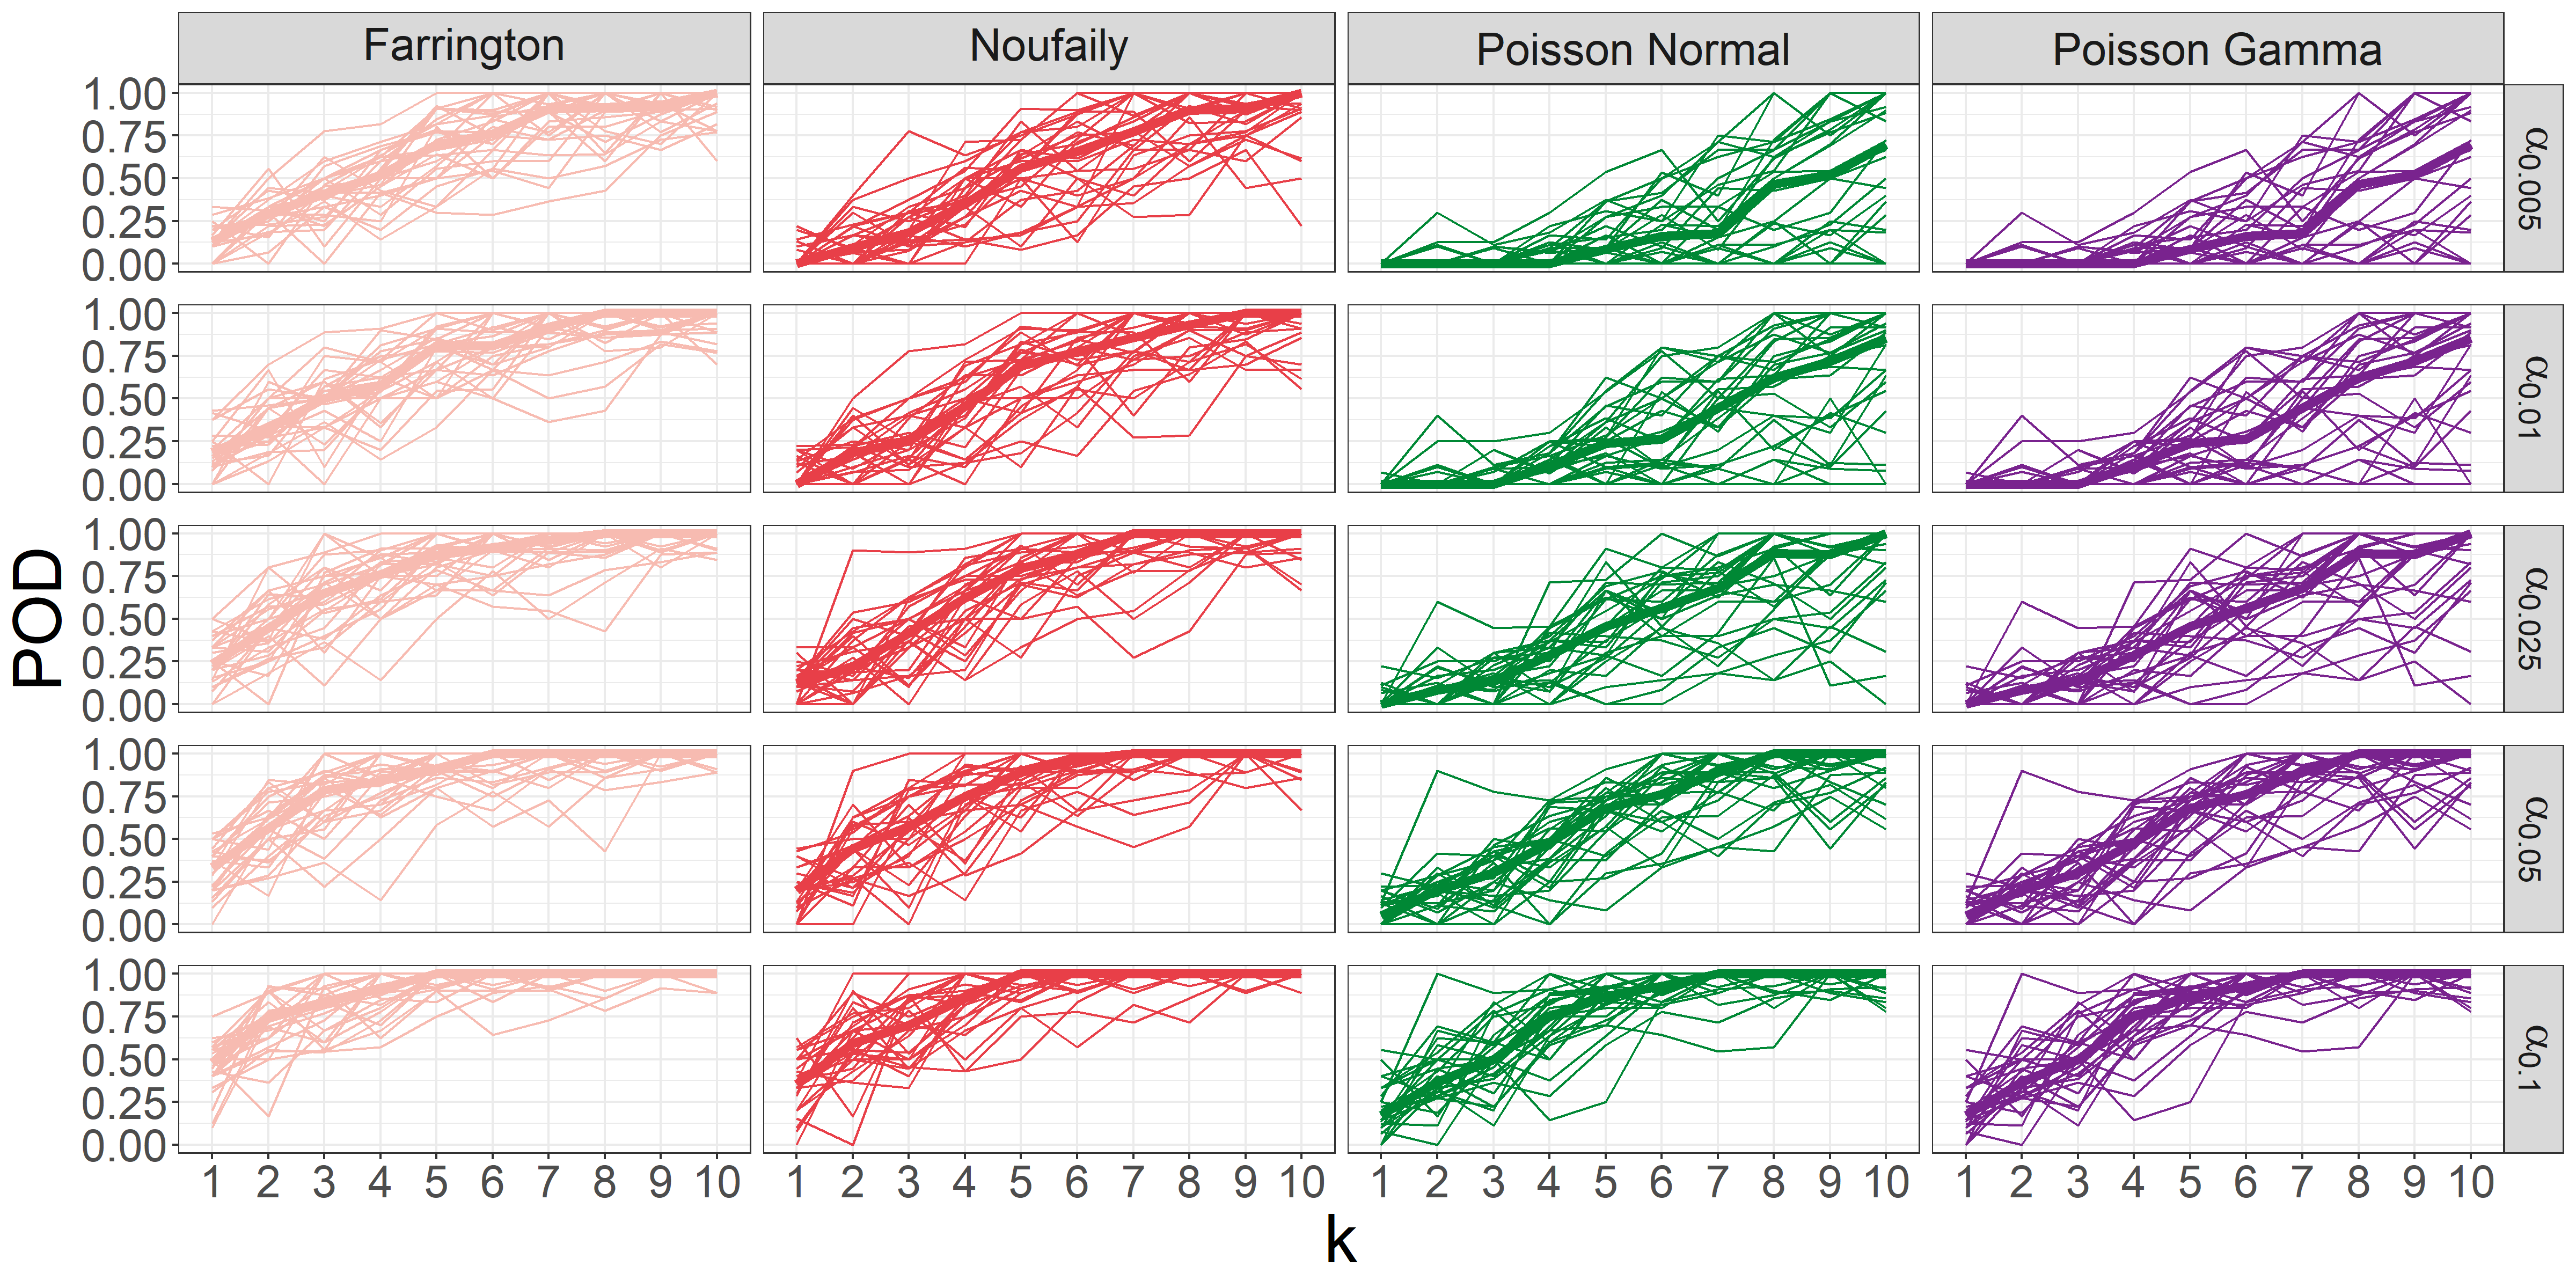
\includegraphics[width=1\linewidth]{../../figures/POD_alpha_methods} \caption{POD of an outbreak of a random size \(v\) drawn from a Poisson distribution with mean equal to \(k\) times the standard deviations of the baseline data for different values of \(\alpha\). The x-axis shows increasing values of \(k\), while the y-axis shows the POD for each scenario along with the median curves (bold) across all 28 scenarios.}\label{fig:PODalphamethods}
\end{figure}

\hypertarget{diagnostic-odds-ratio-1}{%
\subsection{Diagnostic odds ratio}\label{diagnostic-odds-ratio-1}}



\begin{figure}[H]
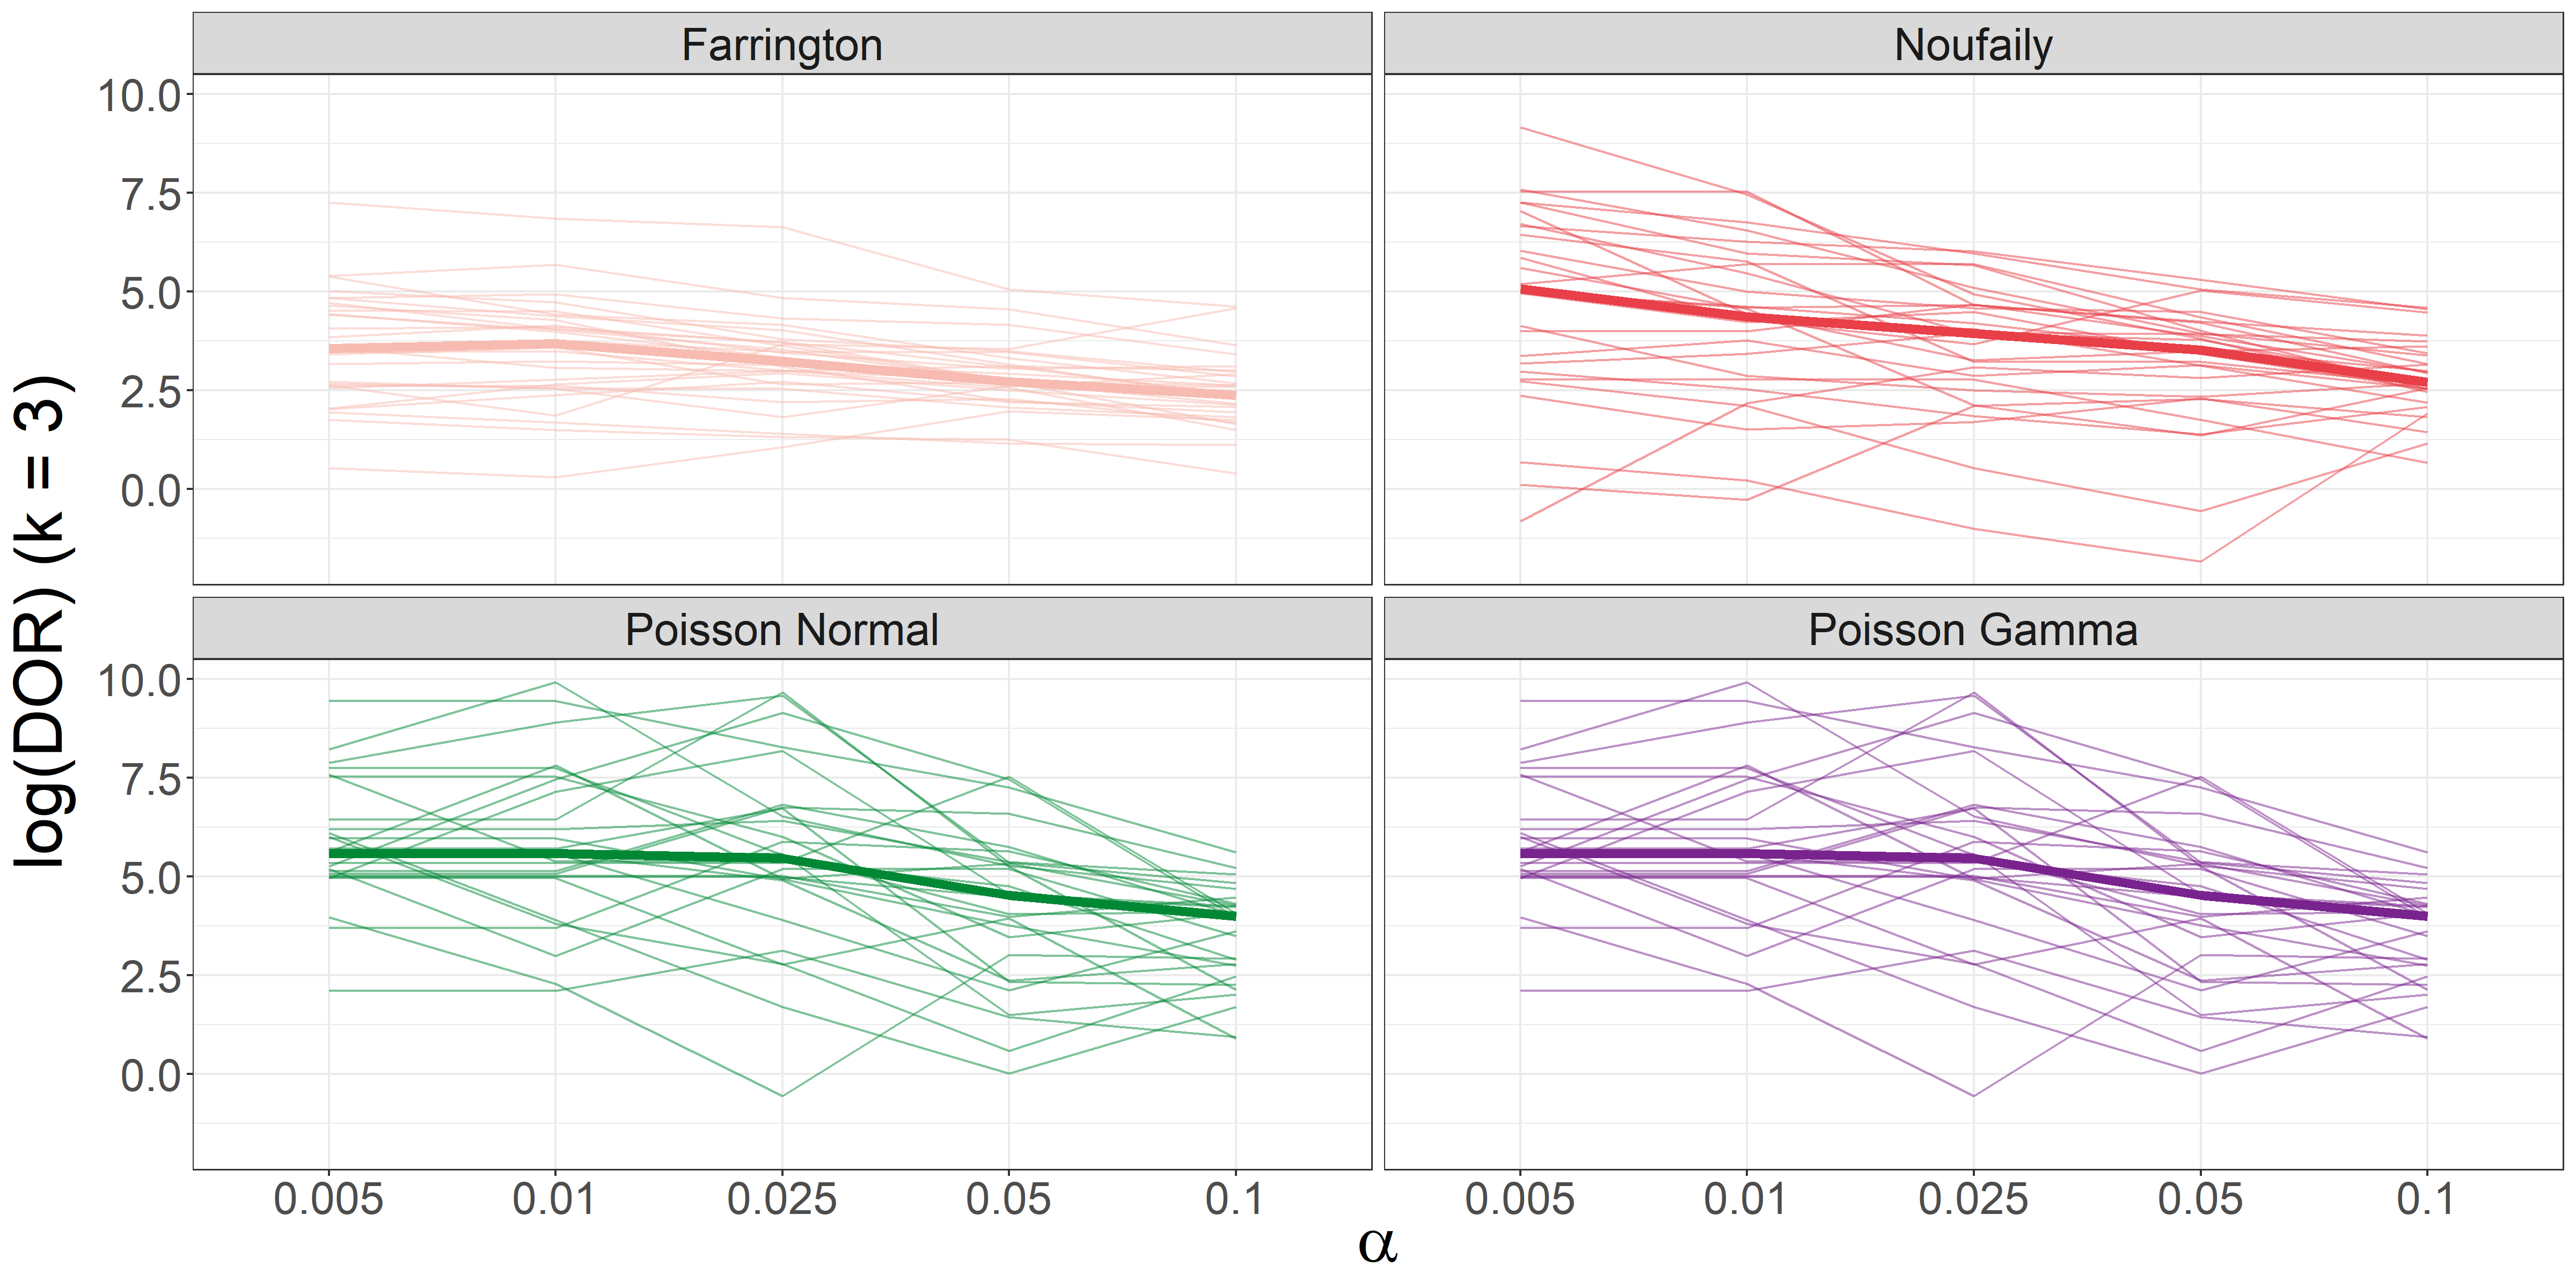
\includegraphics[width=1\linewidth]{../../figures/logDORk3} \caption{Logarithmic DOR of an outbreak of a random size \(v\) drawn from a Poisson distribution with mean equal to \(k\) equal to three times the standard deviations of the baseline data for different values of \(\alpha\). The x-axis shows the different significance levels, \(\alpha\), for the threshold calculations, while the y-axis shows the logarithmic DOR for each scenario along with the median curves (bold) across all 28 scenarios.}\label{fig:logDORk3}
\end{figure}



\begin{figure}[H]
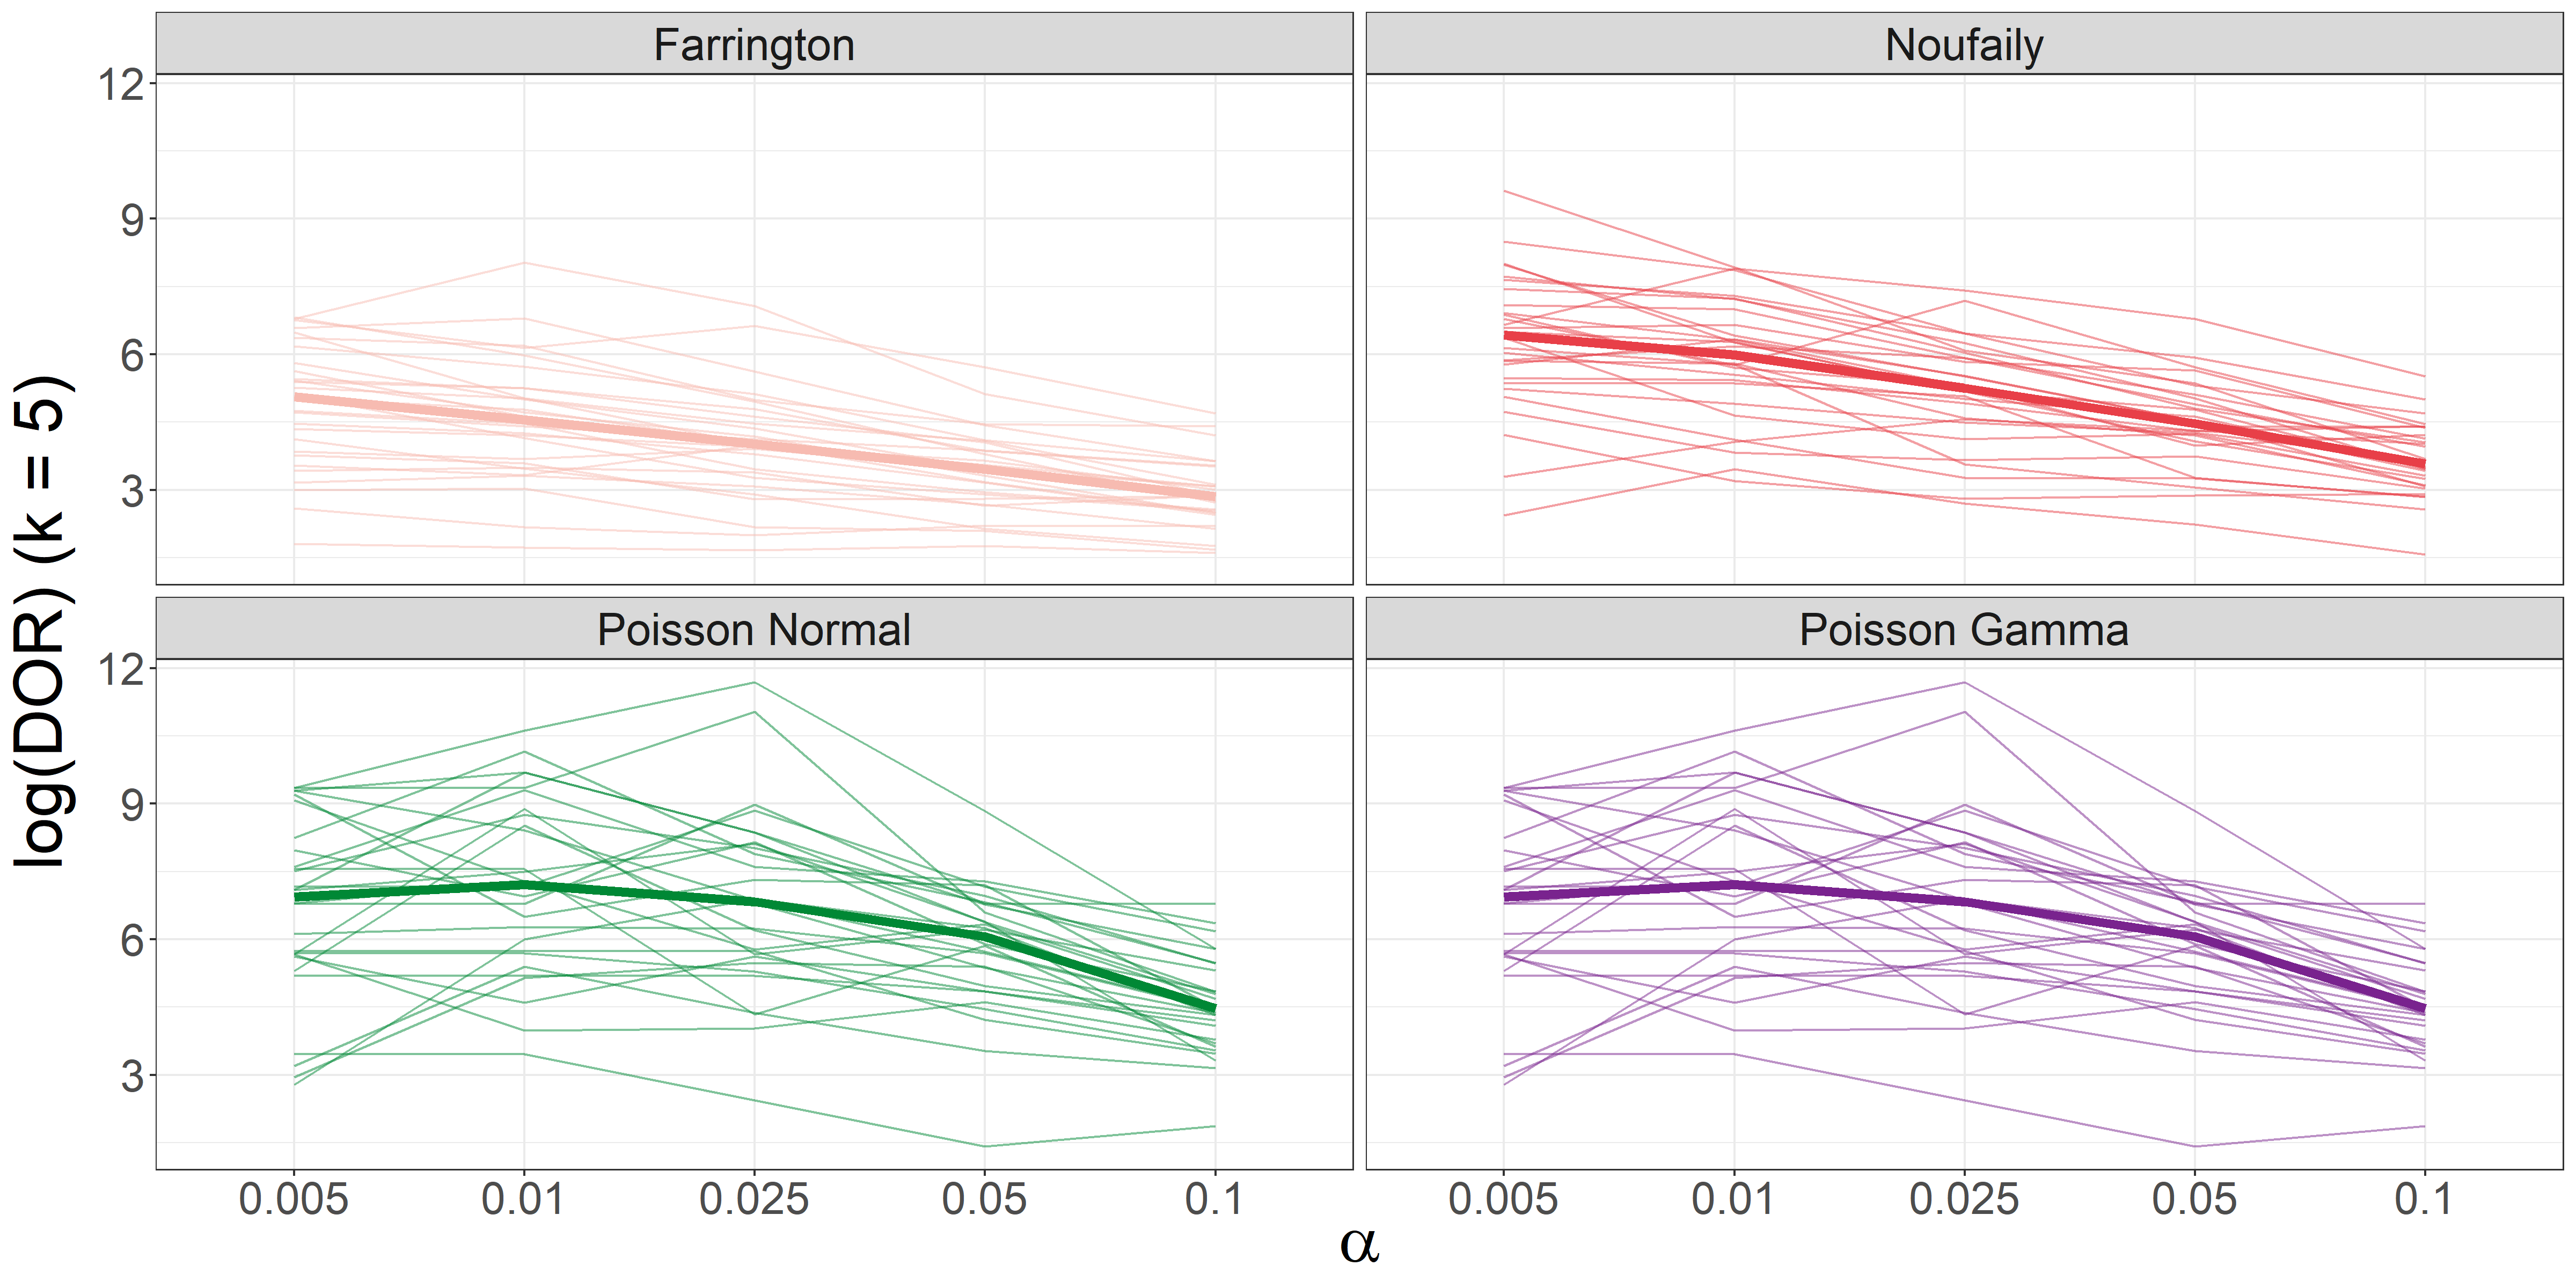
\includegraphics[width=1\linewidth]{../../figures/logDORk5} \caption{Logarithmic DOR of an outbreak of a random size \(v\) drawn from a Poisson distribution with mean equal to \(k\) equal to five times the standard deviations of the baseline data for different values of \(\alpha\). The x-axis shows the different significance levels, \(\alpha\), for the threshold calculations, while the y-axis shows the logarithmic DOR for each scenario along with the median curves (bold) across all 28 scenarios.}\label{fig:logDORk5}
\end{figure}



\begin{figure}[H]
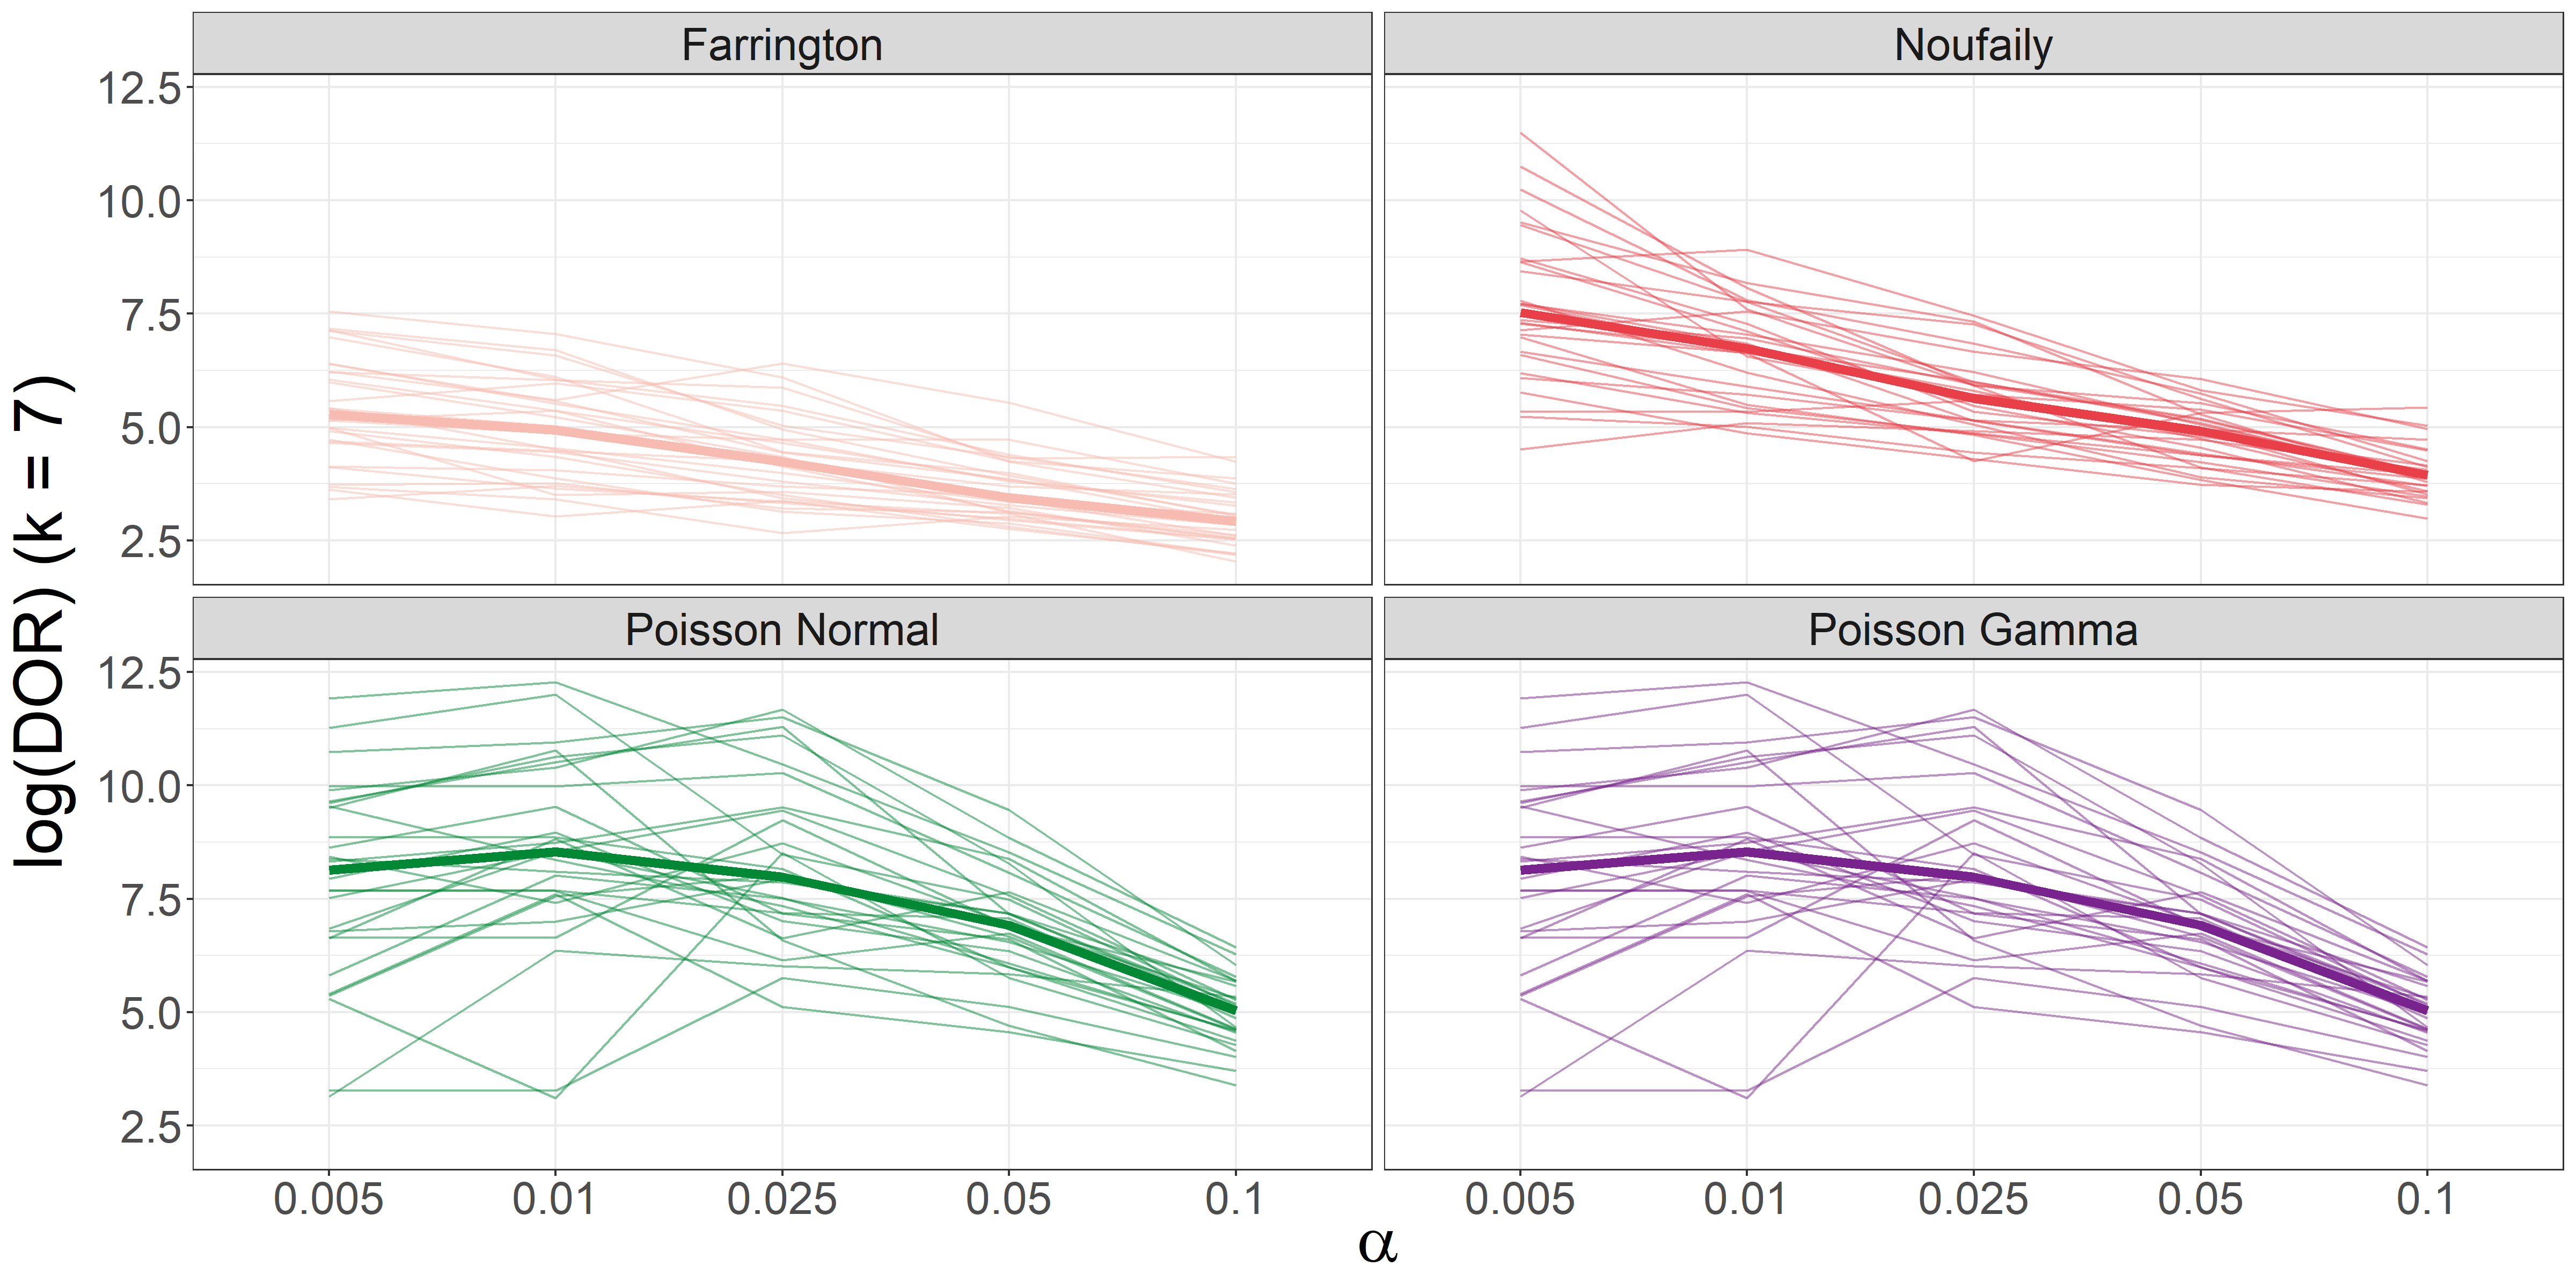
\includegraphics[width=1\linewidth]{../../figures/logDORk7} \caption{Logarithmic DOR of an outbreak of a random size \(v\) drawn from a Poisson distribution with mean equal to \(k\) equal to seven times the standard deviations of the baseline data for different values of \(\alpha\). The x-axis shows the different significance levels, \(\alpha\), for the threshold calculations, while the y-axis shows the logarithmic DOR for each scenario along with the median curves (bold) across all 28 scenarios.}\label{fig:logDORk7}
\end{figure}

\newpage

\renewcommand\refname{References}
\bibliography{mybibfile.bib}


\end{document}
